%%%%%%%%%%%%%%%%%%%%%%%%%%%%%%%%%%%%%%%%%%%%%%%%%%%%%%%%%%%%%%%%%%%%%%%%%
%%   CHAPTER: SELF-SUPPORTING SPACESHIPS
%%%%%%%%%%%%%%%%%%%%%%%%%%%%%%%%%%%%%%%%%%%%%%%%%%%%%%%%%%%%%%%%%%%%%%%%%

\renewcommand{\chapterfolder}{self_support_spaceships/}
\chapterimage{cover/self_support_spaceships}
\chapter{Self-Supporting Spaceships}\label{chp:self_support_spaceships}\index{self-supporting spaceship}


\vspace*{-0.4in}
\epigraph{Figuring out how to achieve a particular behavior makes a pleasant puzzle; actually building the thing is mostly tedious.}{Dean Hickerson}
\vspace*{0.4in}


\noindent Universal computation, covered in the previous chapter, is the first of two major types of universality that often show up in discussions of Conway's Game of Life, and cellular automata in general. The second type of universality is universal construction. Whereas universal computation is the ability to ``compute anything that can be computed'', universal construction could be loosely summarized as the ability to ``construct anything that can be constructed''.

We will cover this topic in much more depth in Chapter~\ref{chp:universal_construction}, but this chapter provides a good preview of the general idea. Indeed, in this chapter we will build spaceships that work by reaching out into a region of empty space in front of themselves and constructing something there. More specifically, self-supporting spaceships (the topic of this chapter) work by manipulating a reaction that moves along a track so as to construct the track in front of itself.


%%%%%%%%%%%%%%%%%%%%%%%%%%%%%%%%
\section{The Silverfish}\label{sec:silverfish}\index{silverfish}
%%%%%%%%%%%%%%%%%%%%%%%%%%%%%%%%

Most self-supporting spaceships rely on a core reaction that moves an object forward with the help of another object that is in its path. One such reaction (simply called the \textbf{31c/240~reaction}) is displayed in Figure~\ref{fig:31c_240_reaction}, in which a Herschel collides with a block in such a way that it moves forward by $31$~cells over the course of $240$ generations.\footnote{We saw another such reaction back in Figure~\ref{fig:17c45_reaction}. We explore the consequences of this reaction a bit later, in Section~\ref{sec:caterpillar}, since building a spaceship out of it is somewhat more technical than the reaction that we use here.} At the same time, the block is moved back by $22$~cells, a second block is created, and two gliders are released.\index{31c/240 reaction}

\begin{figure}[!htb]
	\centering\embedlink{31c_240_reaction}{\vcenteredhbox{\patternimg{0.12}{31c_240_reaction_0}} \vcenteredhbox{\genarrow{240}} \vcenteredhbox{\patternimg{0.12}{31c_240_reaction_240}}}
	\caption{The \textbf{31c/240~reaction}. A Herschel collides with a block so as to move forward by $31$~cells (and move the block back by $22$~cells) over the course of $240$~generations. This reaction also produces a second block (at the top-center) and two gliders as by-products.}\label{fig:31c_240_reaction}
\end{figure}

The first major goal of this chapter is to use this reaction to create a $31c/240$ spaceship, which we call the \textbf{silverfish}. The major obstacles that we will have to overcome are cleaning up the extra objects (blocks and gliders) left behind by the Herschel as it moves, and using the Herschel to create a block in front of itself before it gets there.


\subsection{Herschel Crawlers and Rakes}\label{sec:silverfish_herschel_crawler}

If we place blocks in a straight line with a spacing of $31$ cells, a Herschel is able to crawl along them (via the $31c/240$ reaction of Figure~\ref{fig:31c_240_reaction}) at a speed of $31c/240$. Furthermore, if we place two of these tracks next to each other, we can use one of the output gliders from one of the Herschels to cleanly erase the extra block that is produced by the other Herschel, as illustrated in Figure~\ref{fig:31c_240_herschel_pair}. When we do this, we get a track for two Herschels called a \textbf{reburnable wick}:\index{reburnable wick} a wick that is not used up (but is potentially repositioned and/or rephased) after its fuse (the pair of Herschels) burns through it.

\begin{figure}[!htb]
	\centering
	\patternimglink{0.0885}{31c_240_herschel_pair}
	\caption{A reburnable block wick, along which a pair of Herschels (highlighted in \bgbox{greenpastel}{green}) can move at a speed of $31c/240$. The spark and blocks highlighted in \bgbox{redback}{red} are only temporary---they are destroyed as the Herschels move farther down the track.}\label{fig:31c_240_herschel_pair}
\end{figure}

While a single Herschel pair changes the positions of the blocks in the reburnable wick, a sequence of 31 Herschel pairs would leave them all exactly where they would be if no Herschels burned through them at all.\footnote{After the $31$ Herschel pairs burned through them, each block would actually be moved back $22 \times 31 = 682$ cells. However, since the wick is infinitely long and the blocks are spaced $31$~cells apart, this makes no difference.} This gives us an infinitely-long pattern that moves at a speed of $31c/240$. We now focus on converting this pattern into a \emph{finite} configuration (i.e., a spaceship) that moves at the same speed.

To this end, we need a way of constructing the blocks in front of the Herschel pairs that burn through them. Fortunately, blocks are fairly easy to construct---we can collide spaceships like gliders together so as to synthesize them. Furthermore, the Herschel pairs create gliders as they move, so we ``just'' need to redirect those gliders in front of the Herschels so as to synthesize the blocks.

Unfortunately, getting gliders (or any other spaceships) in front of the Herschel pair is quite tricky, as it does not seem like it should be possible to reflect the gliders that the Herschel pair emits without making use of stationary components like Snarks or other small spaceships (none of which travel at $31c/240$). One technique that works to at least let us send gliders forward (instead of backward, as in Figure~\ref{fig:31c_240_herschel_pair}) is to use the two-glider kickback reaction from Table~\ref{tab:2_glider_synth}. Unfortunately, to make use of this reaction, we have to place even more of these tracks next to each other. One configuration that works is displayed in Figure~\ref{fig:31c_240_forward_rake}---it makes use of six Herschels and six block tracks instead of just two.

We call this pattern a \textbf{forward rake}\index{forward rake} even though it is not \emph{technically} a rake due to its reliance on the supporting block tracks. Since firing gliders backward via these Herschels is so straightforward (they fire gliders backward all on their own, after all), it is not difficult to construct the \textbf{backward rake}\index{backward rake} in Figure~\ref{fig:31c_240_back_rake} that works on this same set of six block tracks (instead of the one that works on two block tracks, which we saw in Figure~\ref{fig:31c_240_herschel_pair}).

These rakes have one big limitation, however---we can only use them to place an output glider on every $31$st lane. If we want to make sure that a glider is fired on a \emph{particular} lane, we need a mechanism for moving the block track (and thus any subsequent rakes) slightly forward or backward. Fortunately, this is also straightforward---the \textbf{rephaser} displayed in Figure~\ref{fig:31c_240_rephaser} moves the block tracks backward by $22$~cells (or equivalently, forward by $9$~cells) simply by having a Herschel burn through each track in such a way that their output gliders annihilate one another. Importantly, since $\mathrm{gcd}(22,31) = 1$, we can use multiple copies of this rephaser so as to make subsequent rakes output gliders on any lanes of our choosing.

\begin{figure}[!htb]
	\centering
	\begin{subfigure}{0.28\textwidth}
		\centering
		\embedlink{31c_240_rakes_and_rephaser}{\gridbox{0.5pt}{\patternimg{0.072}{31c_240_back_rake}}}
		\caption{A backward rake.}\label{fig:31c_240_back_rake}
	\end{subfigure} \ \ \begin{subfigure}{0.28\textwidth}
		\centering
		\patternlink{31c_240_rakes_and_rephaser}{\gridbox{0.5pt}{\patternimg{0.072}{31c_240_rephaser}}}
		\caption{A rephaser.}\label{fig:31c_240_rephaser}
	\end{subfigure} \ \ \begin{subfigure}{0.4\textwidth}
		\centering
		\patternlink{31c_240_rakes_and_rephaser}{\gridbox{0.5pt}{\patternimg{0.072}{31c_240_forward_rake}}}
		\caption{A forward rake.}\label{fig:31c_240_forward_rake}
	\end{subfigure}
	\caption{Rakes and rephasers that crawl along $6$ reburnable block wicks at a speed of $31c/240$. In each case, the $6$ Herschels release $12$ gliders every $240$~generations, and $6$ of those gliders are used to destroy the excess blocks left behind by each Herschel. In (a) the backward rake, $4$ of the gliders collide so as to destroy each other and the other $2$ are released backward. In (b) the rephaser, $2$ gliders are destroyed in a kickback reaction and then the other $4$ are destroyed by colliding into each other. In (c) the forward rake, $4$ kickback reactions are used to destroy $4$ of the gliders, leaving the remaining $2$ gliders to escape to the front.}\label{fig:31c_240_rakes_and_rephaser}
\end{figure}


\subsection{Synthesizing and Destroying Block Tracks}\label{sec:silverfish_synth_destroy_blocks}

Fortunately, even though we now have $6$ block tracks, the problem of constructing the blocks in front of the Herschels is not much trickier than it was when we just had $2$ block tracks. Indeed, we can construct $4$ of these block tracks simply via these rakes and some additional kickback reactions, as illustrated in Figure~\ref{fig:31c_240_track_builder}.

Lining up these kickback reactions and block syntheses is somewhat tricky due to the difficulty of controlling which lanes we produce gliders on when using these tracks. Fortunately, we have complete control of the \emph{timing} of the gliders on these lanes. By delaying Herschels appropriately (and perhaps adding a single row of blocks to a track so as to change the color of the gliders that a Herschel produces) we can create any $2$-glider collision that we like. With this technique we can clean up these six block tracks, just by using even more kickback reactions as illustrated in Figure~\ref{fig:31c_240_track_destroyer}.

\begin{figure}[!htbp]
	\centering
	\begin{subfigure}{\textwidth}
		\centering
		\embedlink{31c_240_track_builder}{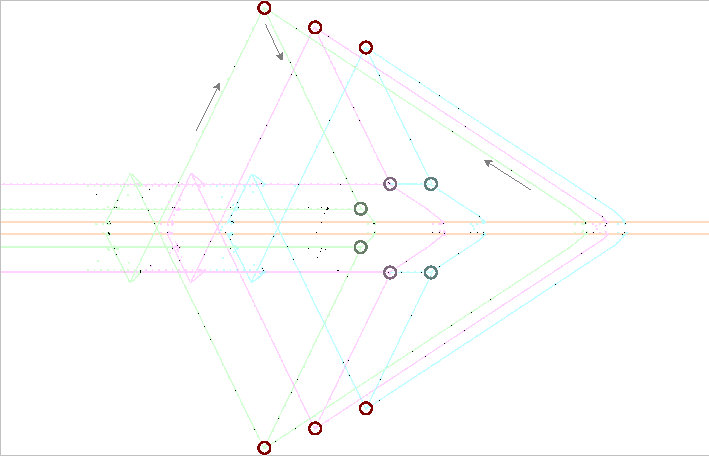
\includegraphics[width=\textwidth]{self_support_spaceships/31c_240_track_builder.pdf}}
		\caption{A configuration of rakes that turns a $2$-block track (highlighted in \bgbox{orangeback2}{orange}) into a $6$-block track.}\label{fig:31c_240_track_builder}
	\end{subfigure} \\[0.2cm]
	\begin{subfigure}{\textwidth}
		\centering
		\embedlink{31c_240_track_destroyer}{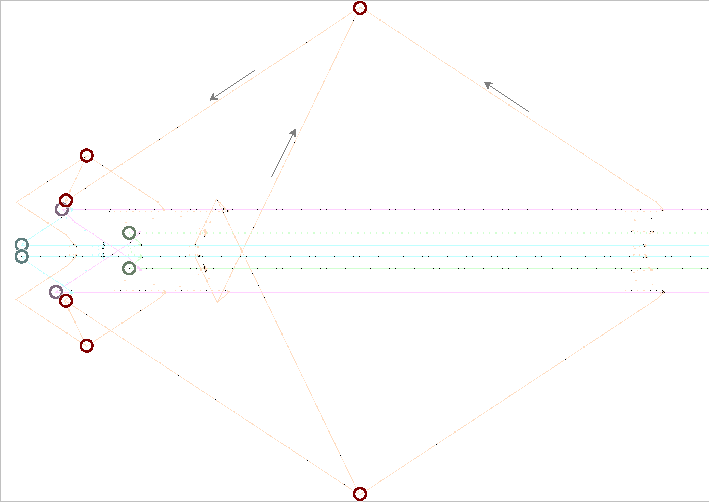
\includegraphics[width=\textwidth]{self_support_spaceships/31c_240_track_destroyer.pdf}}
		\caption{A configuration of rakes that destroys the $6$-block track. Destroying the tracks is actually straightforward, but multiple kickback reactions must be used to clean up the leftover gliders (highlighted in \bgbox{orangeback2}{orange}).}\label{fig:31c_240_track_destroyer}
	\end{subfigure} \\
	\caption{A configuration of rakes that uses multiple kickback reactions (circled in \bgbox{redback}{red}) to position gliders so that they can either (a) synthesize block tracks ahead of the rakes, or (b) destroy the block tracks behind the rakes. The locations where gliders synthesize or destroy the block tracks are circled near the center.}\label{fig:31c_240_builder_destroyer}
\end{figure}

However, we still do not have a method of constructing the two central block tracks at the front of Figure~\ref{fig:31c_240_track_builder}, since there is no way to arrange kickback reactions so as to put gliders in front of the frontmost rakes. While this may seem like an insurmountable problem at first, one solution is to synthesize light, middle, and/or heavyweight spaceships that travel in the same direction as the Herschels, and then bounce gliders off of those rows of xWSSs.

While this approach works, there is an another method that results in the silverfish spaceship being significantly smaller. Instead of bouncing a glider back toward the front of the Herschels so as to synthesize the block track, we convert that glider into a middleweight spaceship via the reaction illustrated in Figure~\ref{fig:g_2h_to_m}. The reason for this is that a middleweight spaceship can stabilize the front of the Herschel track in the exact same way as a block (in fact, one of the Herschel's sparks simply converts the MWSS into a block in the correct position), as illustrated in Figure~\ref{fig:herschel_mwss_stabilize}.

\begin{figure}[!htb]
	\centering
	\begin{subfigure}[b]{0.43\textwidth}
		\centering
		\embedlink{g_2h_to_m}{\vcenteredhbox{\patternimg{0.15}{g_2h_to_m}} \vcenteredhbox{\genarrow{38}} \vcenteredhbox{\patternimg{0.15}{g_2h_to_m_38}}}
		\caption{A way of colliding a glider with two heavyweight spaceships so as to make a perpendicular middleweight spaceship.}\label{fig:g_2h_to_m}
	\end{subfigure} \ \	\ \ \ \begin{subfigure}[b]{0.53\textwidth}
		\centering
		\embedlink{herschel_mwss_stabilize}{\vcenteredhbox{\patternimg{0.08}{herschel_mwss_stabilize}} \vcenteredhbox{\genarrow{98}} \vcenteredhbox{\patternimg{0.08}{herschel_mwss_stabilize_98}} \vcenteredhbox{\genarrow{142}} \vcenteredhbox{\patternimg{0.08}{herschel_mwss_stabilize_240}}}
		\caption{An MWSS stabilizing a Herschel crawler.}\label{fig:herschel_mwss_stabilize}
	\end{subfigure}
	\caption{Some reactions that can be used to stabilize the front of the $31c/240$ Herschel crawler, as long as we can somehow create a parallel double stream of heavyweight spaceships.}\label{fig:silverfish_mwss_reactions}
\end{figure}

The last remaining question before we can piece together all of these reactions is how to create the pair of heavyweight spaceships that are used in Figure~\ref{fig:g_2h_to_m}. The key insight that makes this possible is the fact that we can fire a glider at an HWSS so as to create some debris without affecting the HWSS (after all, heavyweight spaceships are nice and sparky), and then we can fire additional gliders at that debris so as to create another HWSS on the same lane.\footnote{In a sense, we are using a heavyweight spaceship to synthesize itself. It is this self-creation that is really what makes it possible to turn the $31c/240$ reaction into a spaceship.}

One reaction that implements the first half of this process, by creating a toad and a beehive a safe distance from the HWSS when a pair of gliders hits it (without disturbing the HWSS\footnote{That is, this reaction is a Heisenburp.}\index{Heisenburp}), is displayed in Figure~\ref{fig:hwss_toad_beehive}. An unfortunate feature of this reaction is that it relies on two synchronized gliders, and synchronizing the precise time and (especially) position of multiple gliders that are fired from these block tracks is quite tricky. Nevertheless, this synchronization is possible via kickback reactions, and one configuration of rakes that produces the exact glider pair that we need is displayed in Figure~\ref{fig:31c_240_double_gun}.

\begin{figure}[!htb]
	\centering
	\begin{subfigure}[b]{0.28\textwidth}
		\centering
		\embedlink{hwss_toad_beehive}{\begin{tikzpicture}[rotate=-90,transform shape]%
			\node[inner sep=0pt,anchor=south west] (dg) at (0,0) {\vcenteredhbox{\patternimg{0.093}{hwss_toad_beehive_0}} \vcenteredhbox{{\color{black}$\xrightarrow{\scriptsize\rotatebox[origin=c]{90}{\text{\clock{2}{40} 160}}}$}} \vcenteredhbox{\patternimg{0.093}{hwss_toad_beehive_160}}};
			\end{tikzpicture}}
		\caption{A way of colliding two gliders with an HWSS so as to make a beehive and a toad away from the HWSS stream, and without affecting the HWSS.}\label{fig:hwss_toad_beehive}
	\end{subfigure} \ \	\ \ \begin{subfigure}[b]{0.69\textwidth}
		\centering
		\embedlink{31c_240_double_gun}{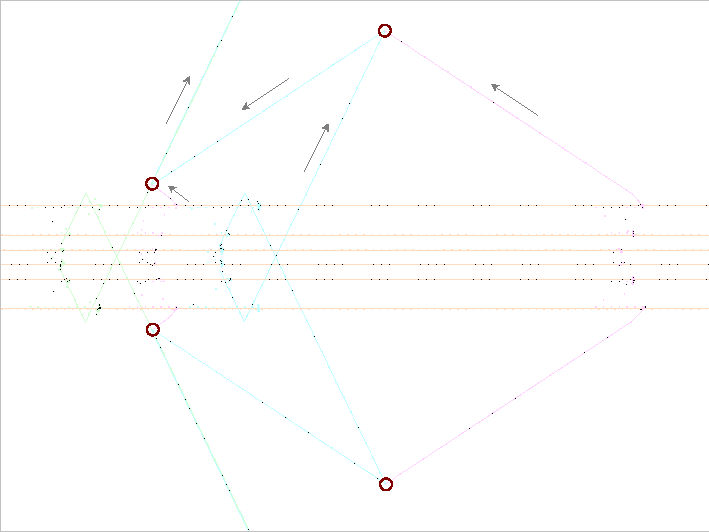
\includegraphics[width=\textwidth]{self_support_spaceships/31c_240_double_gun.pdf}}
		\caption{A configuration of block-crawling rakes that uses some kickback reactions (circled in \bgbox{redback}{red}) to create the synchronized $2$-glider paired needed in (a).}\label{fig:31c_240_double_gun}
	\end{subfigure}
	\caption{The configuration of rakes in (b) sends out a pair of gliders that, when they collide with a heavyweight spaceship as in (a), produce a beehive and a toad. That beehive and toad can then be used as a seed for a slow-salvo synthesis of that heavyweight spaceship.}\label{fig:31c_240_double_gun_at_hwss}
\end{figure}

There are numerous different ways that we could fire gliders at that toad and beehive so as to turn them into a heavyweight spaceship on the correct lane. For the sake of simplicity, we use a slow salvo, since synchronizing the precise time and (especially) position of multiple gliders that are fired from these block tracks is quite tricky (as we saw for just two gliders in Figure~\ref{fig:31c_240_double_gun}). We furthermore just use gliders coming from one of the four possible directions, since (a) the gliders are fired from the $6$-block track, which restricts us to just two directions (i.e., from forward and backward rakes on the block track), and (b) if we further restrict to gliders just coming from forward rakes then it makes the resulting construction of the $31c/240$ spaceship somewhat simpler and more uniform.\footnote{Point (b) here is somewhat subjective---allowing gliders from backward rakes would decrease the number of gliders required, but perhaps increase the spacing needed between the rakes and make their placement somewhat more complicated.} One particular slow salvo of this type that works is displayed in Figure~\ref{fig:hwss_from_toad_beehive}.\footnote{This recipe was produced by a long-running breadth-first search using a script that was written by ConwayLife.com forums user ``oblique''---see \httpsurl{conwaylife.com/forums/viewtopic.php?t=1296}. It was one of the first options to show up that produced an upward HWSS with enough clearance that other HWSSes could safely travel past all the intermediate stages of the slow-salvo construction. It is not necessarily the smallest unidirectional salvo that exists, but it is probably fairly close.}


\subsection{Glider Lanes and More Rakes}\label{sec:silverfish_more_rakes}

At this point, we have essentially everything that we need to construct a $31c/240$ spaceship. However, the spaceship that results from combining the various reactions and patterns that we have developed in this section ends up being monstrously large, so it is worthwhile to spend some time thinking about how we can reduce its size prior to assembling it.

The majority of this spaceship's length will come from the multi-step process needed to synthesize the heavyweight spaceship pair on each of its sides via the slow salvo of Figure~\ref{fig:hwss_from_toad_beehive}.\footnote{Similarly, the majority of its width comes from how close to the front of the spaceship we can put the first forward rake.} Indeed, implementing this synthesis requires $13$ gliders and thus $13$ forward rakes. Furthermore, we need to use between $0$ and $30$ rephasers before each of those rakes to make sure the gliders that they emit are positioned on the correct mod~$31$ lane.

\begin{figure}[!htb]
	\centering\raisebox{-0.49\height}{\begin{tikzpicture}[scale=0.5, every node/.style={transform shape}]%
		\node[inner sep=0pt,anchor=south west] at (0,0) {\embedlink{hwss_from_toad_beehive}{\patternimg{0.182}{hwss_from_toad_beehive}}};
		
		\colorletternode{green}{9.89}{6.3}{1}
		\colorletternode{green}{10.43}{10.8}{2}
		\colorletternode{green}{8.77}{8.53}{3}
		\colorletternode{green}{7.88}{7.7}{4}
		\colorletternode{green}{9.16}{5.05}{5}
		\colorletternode{green}{6.68}{7.48}{6}
		\colorletternode{green}{8.08}{4.49}{7}
		\colorletternode{green}{5.07}{8.45}{8}
		\colorletternode{green}{6.08}{5.81}{9}
		\colorletternode{green}{7.21}{3.3}{10}
		\colorletternode{green}{4.45}{5.42}{11}
		\colorletternode{green}{3.14}{5.83}{12}
		\colorletternode{green}{6.12}{2.63}{13}
		\end{tikzpicture}} \patternlink{hwss_from_toad_beehive}{\vcenteredhbox{\gliderarrow{13}} \vcenteredhbox{\patternimg{0.091}{hwss_from_toad_beehive_13}}}
	\caption{A $13$-glider slow salvo that turns the configuration of a beehive and toad from Figure~\ref{fig:hwss_toad_beehive} back into an HWSS on the same lane as the HWSS that was used to create them.}\label{fig:hwss_from_toad_beehive}
\end{figure}

In order to reduce the number of rephasers needed, and thus reduce the spaceship's length, we now introduce several other forward rakes that emit gliders on different lanes. These rakes, which are displayed in Figure~\ref{fig:31c_240_forerakes},\footnote{This collection of rakes is by no means exhaustive. See Exercises~\ref{exer:self_support_spaceships_r4l1}--\ref{exer:self_support_spaceships_r3l28}, and there are many others known as well (and probably quite a few others waiting to be found). The rakes given in Figure~\ref{fig:31c_240_forerakes} are pretty good at hitting each mod~$31$ lane efficiently, though.} work in one of three different ways:\smallskip

\begin{itemize}
	\item by using multiple copies of the two-glider kickback reaction (as in Figure~\ref{fig:R6L17}),\footnote{Each pair of kickback reactions that we use in this way has the net effect of adding $2$ rephaser lengths to the rake and increasing its output lane number by $16$ (mod $31$)---see Exercise~\ref{exer:self_support_spaceships_r4l1}.}\smallskip
	
	\item by using the two-glider synthesis of a traffic light and a glider from Table~\ref{tab:2_glider_synth}, and then using another glider or two to clean up the traffic light (as in Figure~\ref{fig:R6L6}), or\smallskip
	
	\item by using two gliders to synthesize a small object that can be used to release a glider on another lane when it is destroyed (as in Figures~\ref{fig:31c_240_forerakes}(a) and~(b)).\smallskip
\end{itemize}

In order to help us keep track of where each of these rakes emits a glider, we name them according to what mod~$31$ lane they fire a glider on (relative to the original forward rake that we saw in Figure~\ref{fig:31c_240_forward_rake}, which we say fires on lane~$0$) and the number of Herschels that are used on each block track. Specifically, their names have the form
\[
\text{\texttt{R<number of Herschels>L<lane number>}},
\]
so that the original rake from Figure~\ref{fig:31c_240_forward_rake}, for example, is called \texttt{R1L0} (it uses a single Herschel on each block track and produces a glider on lane~0).\footnote{The ``\texttt{R}'' in this naming scheme stands for the fact that the rake has approximately the same length as this number of \textbf{r}ephasers, and the ``\texttt{L}'' stands for ``\textbf{l}ane''.}

\begin{figure}[!htb]
	\centering
	\begin{minipage}{0.3\textwidth}
		\begin{subfigure}{\linewidth}
			\centering
			\gridbox{0.5pt}{\patternimglink{0.0975}{R2L23}}
			\caption{\texttt{R2L23}\index{R2L23}}\label{fig:R2L23}
		\end{subfigure} \\[0.1cm] \begin{subfigure}{\linewidth}
			\centering
			\gridbox{0.5pt}{\patternimglink{0.0975}{R2L25}}
			\caption{\texttt{R2L25}\index{R2L25}}\label{fig:R2L25}
		\end{subfigure}
	\end{minipage} \ \ \ \begin{subfigure}{0.66\textwidth}
		\centering
		\gridbox{0.5pt}{\patternimglink{0.072}{R6L17}}
		\caption{\texttt{R6L17}\index{R6L17}}\label{fig:R6L17}
	\end{subfigure} \\[0.1cm]
	\begin{subfigure}{0.3\textwidth}
		\centering
		\gridbox{0.5pt}{\patternimglink{0.0975}{R1L0}}
		\caption{\texttt{R1L0}\index{R1L0}}\label{fig:R1L0}
	\end{subfigure} \ \ \ \begin{subfigure}{0.66\textwidth}
		\centering
		\gridbox{0.5pt}{\patternimglink{0.06444285714}{R6L6}}
		\caption{\texttt{R6L6}\index{R6L6}}\label{fig:R6L6}
	\end{subfigure}
	\caption{Several forward rakes that crawl along a six-block track and emit gliders on different lanes mod~$31$. The forward rake from Figure~\ref{fig:31c_240_forward_rake} is the one displayed here at the bottom-left, called \texttt{R1L0}.}\label{fig:31c_240_forerakes}
\end{figure}

The ``\texttt{R}'' piece of this naming scheme is useful both as a measure of how long the rake is (e.g., it tells us that \texttt{R6L17} is roughly three times as long as \texttt{R2L25}) and also for computing the mod~$31$ output glider lane of subsequent rakes. Indeed, a single rephaser (i.e., one Herschel on each block track) changes the output lane of subsequent gliders by $-22$ (or equivalently, by $+9$) mod $31$, so a rake with name \texttt{R<m>L<n>} adjusts the output lane of subsequent gliders by $+9m$ (mod $31$). For example, \texttt{R6L21} increases the output lane of subsequent gliders by $9 \times 6 = 54 \equiv 23$ (mod $31$).

With these rakes in hand, we can fire gliders on particular mod~$31$ lanes much more efficiently than we could previously. For example, placing a glider on lane~$22$ (when the block track is currently aligned to lane~$0$) via just the rakes and rephaser from Figure~\ref{fig:31c_240_rakes_and_rephaser} would require $30$~rephasers followed by the forward rake \texttt{R1L0}. However, a much more efficient way of firing a glider on lane~$22$ is to use just $4$~rephasers and then the forward rake \texttt{R6L17} (for a total length of $4 + 6 = 10$ Herschels per track, instead of $30 + 1 = 31$ Herschels per track). A summary of the most efficient rake to use to place a glider on each mod~$31$ lane is provided in Table~\ref{tab:silverfish_forward_rakes}.

\begin{table}[!htbp]
	\centering
	\begin{tabular}{c l | c l | c l | c l}
		\toprule
		Lane & Cheapest Rake & Lane & Rake & Lane & Rake & Lane & Rake \\ \midrule
		0 & \texttt{R1L0} & 9 & 1 + \texttt{R1L0} & 18 & 2 + \texttt{R1L0} & 27 & 3 + \texttt{R1L0} \\
		1 & 1 rephaser + \texttt{R2L23} & 10 & 2 + \texttt{R2L23} & 19 & 3 + \texttt{R2L23} & 28 & 4 + \texttt{R2L23}\\
		2 & 3 rephasers + \texttt{R6L6} & 11 & 4 + \texttt{R6L6} & 20 & 5 + \texttt{R6L6} & 29 & 6 + \texttt{R6L6} \\
		3 & 1 rephaser + \texttt{R2L25} & 12 & 2 + \texttt{R2L25} & 21 & 3 + \texttt{R2L25} & 30 & 4 + \texttt{R2L25} \\
		4 & 2 rephasers + \texttt{R6L17} & 13 & 3 + \texttt{R6L17} & 22 & 4 + \texttt{R6L17} & & \\
		5 & 4 rephasers + \texttt{R1L0} & 14 & 5 + \texttt{R1L0} & 23 & \texttt{R2L23} & & \\
		6 & \texttt{R6L6} & 15 & 1 + \texttt{R6L6} & 24 & 2 + \texttt{R6L6} & & \\
		7 & 7 rephasers + \texttt{R6L6} & 16 & 8 + \texttt{R6L6} & 25 & \texttt{R2L25} & & \\
		8 & 5 rephasers + \texttt{R2L25} & 17 & \texttt{R6L17} & 26 & 1 + \texttt{R6L17} & & \\
		\bottomrule
	\end{tabular}
	\caption{A summary of the shortest forward rakes that can be used to put a glider on a given lane (mod $31$). For example, the shortest configuration of rephasers and forward rakes that can put a glider on lane~22 (when currently aligned to lane~0) consists of 4 rephasers followed by \texttt{R6L17}. Indeed, that configuration has a total length that is roughly the same as that of $6 + 4 = 10$ rephasers, and no other way of using rephasers and forward rakes is shorter.}\label{tab:silverfish_forward_rakes}
\end{table}


\subsection{Completing the Silverfish}\label{sec:silverfish_completed}

We now proceed with construction of the silverfish. At the front of the spaceship we use the track-building component that we built in Figure~\ref{fig:31c_240_track_builder} (with the understanding that we will still have to construct the two central block tracks somehow), and at the back of the spaceship we use the track-destroying component that we built in Figure~\ref{fig:31c_240_track_destroyer}. Right behind the track-building component, we place a forward rake that is aimed at a parallel stream of heavyweight spaceship pairs as in Figure~\ref{fig:g_2h_to_m}, which create middleweight spaceships to stabilize the two central block tracks as in Figure~\ref{fig:herschel_mwss_stabilize}.

The remainder of the silverfish is made up of forward rakes that synthesize the stream of heavyweight spaceship pairs, using the mechanisms of Figures~\ref{fig:31c_240_double_gun_at_hwss} and~\ref{fig:hwss_from_toad_beehive}. Indeed, after using the double gun from Figure~\ref{fig:31c_240_double_gun} to create a beehive and toad, we want to create $13$~gliders on the following sequence of lanes, as indicated by Figure~\ref{fig:hwss_from_toad_beehive}:\footnote{We actually have some flexibility in which lanes we use here---see Exercise~\ref{exer:silverfish_list_of_lanes}.}\label{page:silverfish_lanes}
\[
\text{\texttt{0, 11, 8, 7, 29, 13, 1, 19, 8, 0, 14, 22, 2}.}
\]
We can place gliders on these lanes by repeatedly using Table~\ref{tab:silverfish_forward_rakes} and keeping track of what lane the block tracks are currently synchronized to. After the two-glider rake from Figure~\ref{fig:31c_240_double_gun}, the block tracks are synchronized to lane~7. We then place $13$ more rakes as follows:\smallskip

\begin{itemize}
	\item First, we want to fire a glider 24 (mod~31) lanes up from the current lane, on lane~0. Table~\ref{tab:silverfish_forward_rakes} tells us that the most efficient way to do this is to use $2$~rephasers and then \texttt{R6L6}. Since this places $8$ Herschels on each track, it synchronizes the block tracks to lane $7 + (9 \times 8) = 79 \equiv 17$ (mod~$31$).\smallskip
	
	\item Next, we want to fire a glider $6$ lanes down (i.e., $25$ lanes up) from here on lane $11$ mod $31$. Table~\ref{tab:silverfish_forward_rakes} tells us that the most efficient way to do this is to use \texttt{R2L25}. Since this places $2$ Herschels on each track, it synchronizes the tracks to lane $17 + (9 \times 2) = 35 \equiv 4$ (mod~$31$).\smallskip
	
	\item Next, we want to fire a glider $4$ lanes up from here on lane $8$. Table~\ref{tab:silverfish_forward_rakes} tells us that the most efficient way to do this is to use $2$~rephasers followed by \texttt{R6L17}. Since this places $8$ Herschels on each track, it synchronizes the tracks to lane $4 + (9 \times 8) = 76 \equiv 14$ (mod~$31$).\smallskip
\end{itemize}

If we continue in this way, we quickly arrive at the following sequence of rakes and rephasers that should be placed along the $6$-block track so as to synthesize one of the heavyweight spaceships that we need beside it:\footnote{The timing of most of these rakes and rephasers does not matter, so we can simply pack them as tightly together as possible. However, the final \texttt{R6L6} has to be delayed slightly so that the HWSS it created arrives at the front double rake at the correct time.}\label{page:silverfish_rake_seq}
\begin{gather*}
	\text{\texttt{double rake, 2 rephasers, R6L6, R2L25, 2 rephasers, R6L17, 2 rephasers, R6L6,}} \\
	\text{\texttt{4 rephasers, R1L0, R6L6, 3 rephasers, R6L6, 1 rephaser, R2L23, R2L25,}} \\
	\text{\texttt{4 rephasers, R2L25, 3 rephasers, R2L25, 1 rephaser, R6L6, R2L25.}}
\end{gather*}

If we use two copies of this entire sequence of rakes and rephasers (since we need to synthesize two heavyweight spaceships on each side of the block track), we finally get a complete $31c/240$ orthogonal spaceship,\footnote{Created by Chris Cain, Dave Greene, and Adam P. Goucher in May 2020.} which is displayed in Figure~\ref{fig:silverfish}. Despite its massive size of $215{\thousep}338$ live cells and $11{\thousep}970 \times 48{\thousep}047$ bounding box, it is the smallest known $31c/240$ spaceship.\footnote{Actually, there are some modifications of it that can reduce its size a bit---see Exercise~\ref{exer:silverfish_backward_glider_destroy}.}

\begin{figure}[!htbp]
	\centering
	\embedlink{silverfish}{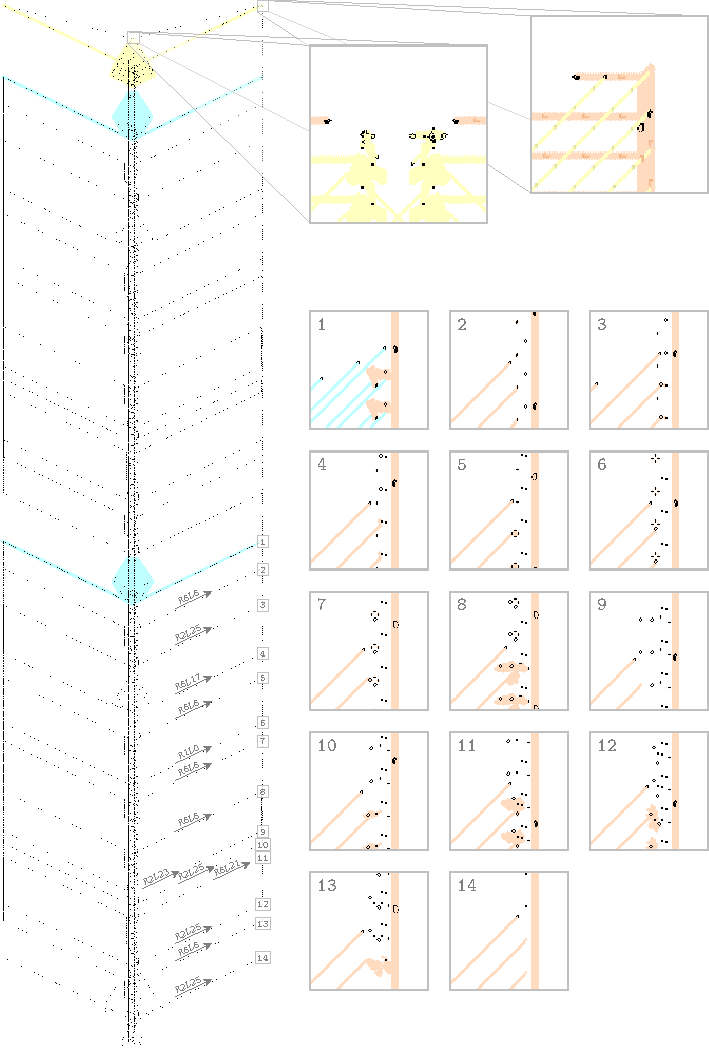
\includegraphics[width=\textwidth]{self_support_spaceships/silverfish.pdf}}
	\caption{The \textbf{silverfish}: a $31c/240$ orthogonal spaceship oriented so that it travels up. The track-building mechanism from Figure~\ref{fig:31c_240_track_builder} is highlighted in \bgbox{yellowback2}{yellow}, a track-destroying mechanism like the one from Figure~\ref{fig:31c_240_track_destroyer} is highlighted in \bgbox{magentaback}{magenta}, and the double-glider forward rakes from Figure~\ref{fig:31c_240_double_gun} are highlighted in \bgbox{aquaback}{aqua}. The remaining un-highlighted rakes implement the 13-step slow salvo synthesis of a heavyweight spaceship from Figure~\ref{fig:hwss_from_toad_beehive}.}\label{fig:silverfish}
\end{figure}


% Nivasch article: http://www.gabrielnivasch.org/fun/life/caterpillar
%%%%%%%%%%%%%%%%%%%%%%%%%%%%%%%%
\section{The Caterpillar}\label{sec:caterpillar}\index{caterpillar}
%%%%%%%%%%%%%%%%%%%%%%%%%%%%%%%%

We saw another reaction that can be used to construct a self-supporting spaceship way back in Figure~\ref{fig:17c45_reaction}: a blinker can be used to move a pi-heptomino forward by $17$~cells over the course of $45$~generations (while just repositioning, not destroying, the blinker). By placing a row of blinkers with a spacing of $17$~cells as in Figure~\ref{fig:reburnable_blinker_wick}, we thus get a reburnable blinker wick that a pi-heptomino can burn through.

\begin{figure}[!htb]
	\centering
	\patternimglink{0.075}{reburnable_wick}
	\caption{A reburnable blinker wick, along which a pi-heptomino fuse (highlighted in \bgbox{greenpastel}{green}) can move at a speed of $17c/45$. The cells displayed in \bgbox{redback}{red} make up a large spark that simply dies without affecting anything else.}\label{fig:reburnable_blinker_wick}
\end{figure}

A single pi-heptomino shifts the blinker wick backward by $6$~cells and rephases it,\footnote{Since the blinker wick is infinitely long, it is perhaps better to think of the pi-heptomino as shifting the wick forward by $11$~cells and \emph{not} rephasing it.} so if we were to place 34 pi-heptominoes on this reburnable wick then it would be moved back by $6 \times 34 = 204$ cells, which, due to the spacing of the blinkers, leaves them all exactly where they would be if no pi-heptominoes burned through them at all.\footnote{If we used just $17$ pi-heptominoes instead, the blinkers would return to their original positions, but in the opposite phases.} This gives us an infinitely-long pattern that moves at a speed of $17c/45$. Our goal is to turn this into a finite configuration (i.e., a spaceship) called the \textbf{caterpillar} that moves at the same speed, just like we turned the Herschel-crawling reaction of Figure~\ref{fig:31c_240_herschel_pair} into the $31c/240$ silverfish spaceship.

To this end, we need a way of constructing the blinkers in front of the pi-heptominoes that burn through them, and also a way of cleaning them up behind those pi-heptominoes. Fortunately, most of the same ideas that we used when constructing the silverfish still apply: we can use multiple pi-heptominoes on multiple reburnable blinker wicks to create rakes, we can use gliders to clean up the blinker trails, and we can use parallel xWSS streams to help us synthesize the front ends of the blinker wicks.

Most of the details of this construction are quite similar to what they were for the $31c/240$ silverfish, so we omit many of them. Instead, we just focus on two parts of the construction where the details do change considerably.


\subsection{Pi-Crawler Rakes}\label{sec:caterpillar_pi_rakes}\index{pi crawler}

The first key difference between the Herschel crawler of Figure~\ref{fig:31c_240_herschel_pair} and the pi crawler that we are now using is that the pi crawler does not emit any gliders on its own. Fortunately, it does create a large spark, and we can collide two of those sparks without much effort so as to create a backward rake, as illustrated in Figure~\ref{fig:pi_backward_rake}. Creating a forward rake that travels along this same pair of blinker tracks is a bit trickier, but can be done via six pi crawlers (three per track), as in Figure~\ref{fig:pi_forward_rake}.

\begin{figure}[!htbp]
	\centering
	\begin{tabular}{@{}cc@{}}
		\begin{subfigure}{0.44\textwidth}
			\patternimglink{0.099}{pi_backward_rake}
			\caption{A backward pi-crawler rake.}\label{fig:pi_backward_rake}
		\end{subfigure} &
		\begin{subfigure}{0.535\textwidth}
			\patternimglink{0.099}{pi_forward_rake}
			\caption{A forward pi-crawler rake.}\label{fig:pi_forward_rake}
		\end{subfigure}
	\end{tabular}
	\caption{A pair of p$45$ (a) backward and (b) forward rakes that crawl along a pair of blinker tracks that are separated by $32$~cells.}\label{fig:pi_rakes}
\end{figure}

While the blinker tracks that these rakes use have the same spacing as each other ($32$ cells), the relative phases of those blinker tracks are different. As a result, it is not possible to place a forward rake directly behind a backward rake, or vice-versa, unless we rephase one of the tracks. Fortunately, we can always properly rephase the tracks by simply inserting additional pi crawlers on one of them, since $\mathrm{gcd}(11,34) = 1$.\footnote{This is directly analogous to how we could always properly rephase the six-block track in the silverfish since $\mathrm{gcd}(9,31) = 1$.}

With that technicality out of the way, we can then place a forward rake on the same pair of tracks behind a backward rate so that their gliders collide and synthesize other objects. For example, we can use these rakes to synthesize and/or destroy additional blinker tracks, as illustrated in Figure~\ref{fig:blinker_trail_synth}. By adjusting the number of pi~rephasers that we use on each track, as well as the relative timing of the forward and backward rakes, we can adjust this reaction to even synthesize a pair of blinker trails that are $32$ cells apart, thus allowing additional rakes to travel along them (see Exercise~\ref{exer:two_pi_tracks_synth_spacing}).

\begin{figure}[!htbp]
	\centering
	\patternimglink{0.111}{blinker_trail_synth}
	\caption{A backward rake (highlighted in \bgbox{aquaback}{aqua}) followed by fourteen rephaser pis (highlighted in \bgbox{yellowback2}{yellow}) that allow a forward rake (highlighted in \bgbox{greenpastel}{green}) to use the same pair of blinker tracks. Those two rakes synthesize a parallel blinker track, which is then destroyed by a third rake (highlighted in \bgbox{magentaback}{magenta}).}\label{fig:blinker_trail_synth}
\end{figure}

We can thus use a single pair of blinker tracks to create as many additional pairs of blinker tracks as we like. Furthermore, those tracks can all clean up after each other, by using rakes to fire gliders at each other so as to destroy the blinkers. All that remains is to synthesize the front of the very first pair of blinker tracks.


\subsection{Helices}\label{sec:caterpillar_helices}\index{helix}

Just as was the case with the silverfish, synthesizing the front of the track is the trickiest part of the caterpillar. Our goal is to use rakes on blinker track pairs to synthesize xWSSes that reach out in front so as to then synthesize the front of the first pair of blinker tracks. However, there is one additional wrinkle here that was not present in the silverfish: because the $17c/45$ reaction that we are using travels faster than $c/4$,\footnote{Unlike the $31c/240$ reaction at the heart of the silverfish, which is slower than $c/4$.} we cannot fire gliders forward at those xWSSes to change their direction (we used this trick from Figure~\ref{fig:g_2h_to_m} at the top-right corner of the silverfish in Figure~\ref{fig:silverfish}).

The way around this problem is to use a \textbf{helix}:\footnote{The name ``helix'' comes from the helical shape that these patterns often end up having---see the upcoming Figure~\ref{fig:caterpillar_helix}.} a configuration of xWSSes that has a burning front end that causes it to (a) travel at a speed slower than $c/2$ (in our case, we want a speed of $17c/45$), and (b) periodically fire gliders off to at least one side. One way to make a helix is to have a glider do the burning---the three reactions displayed in Figure~\ref{fig:helix_operations} show how a glider can destroy and be repositioned (and possibly duplicated) by small xWSS flotillae.\footnote{These reactions were found by Paul Callahan's \emph{gencols}\index{gencols} search program---see \httpsurl{conwaylife.com/wiki/LifeWiki:Life_links\#Downloadable_Computation_and/or_Search_Software}.}\index{gencols}

\begin{figure}[!htb]
	\centering
	\begin{subfigure}[b]{0.475\textwidth}
		\centering
		\embedlink{helix_operations}{\vcenteredhbox{\patternimg{0.125}{helix_shift_0}} \vcenteredhbox{\genarrow{20}} \vcenteredhbox{\patternimg{0.125}{helix_shift_20}}}
		\caption{Shifting a glider by $(10,13)$ in $20$ generations.}\label{fig:helix_shift}
	\end{subfigure} \quad \ \ \ \begin{subfigure}[b]{0.475\textwidth}
		\centering
		\patternlink{helix_operations}{\vcenteredhbox{\patternimg{0.11316568047}{helix_reflect_0}} \vcenteredhbox{\genarrow{39}} \vcenteredhbox{\patternimg{0.11316568047}{helix_reflect_39}}}
		\caption{Reflecting a glider in $39$ generations.}\label{fig:helix_reflect}
	\end{subfigure}\\[0.3cm]
	\begin{subfigure}[b]{\textwidth}
		\centering
		\patternlink{helix_operations}{\vcenteredhbox{\patternimg{0.1}{helix_duplicate_0}} \vcenteredhbox{\genarrow{8}} \vcenteredhbox{\patternimg{0.1}{helix_duplicate_8}} \vcenteredhbox{\genarrow{54}} \vcenteredhbox{\patternimg{0.1}{helix_duplicate_62}}}
		\caption{Reflecting a glider in $62$ generations, while duplicating it. Delaying the final pair of xWSSes delays the output gliders by the same amount, without affecting their position.}\label{fig:helix_duplicate}
	\end{subfigure}
	\caption{Some methods of colliding a glider with xWSS flotillae so as to (a) move the glider, (b) reflect it, and (c) duplicate it. The spark displayed in \bgbox{redback}{red} dies off in another 9~generations.}\label{fig:helix_operations}
\end{figure}

By stringing these reactions together, we can create helices that a glider burns through at any speed of our choosing. For example, the helix displayed in Figure~\ref{fig:caterpillar_helix} takes $270$~generations to push a glider forward orthogonally by $102$~cells, giving it a speed of $102c/270 = 17c/45$---exactly the speed that we need for the caterpillar spaceship.

It was not just a lucky coincidence that we were able to create a helix of the desired $17c/45$ speed via these three reactions---we can use them to make an orthogonal helix with the same basic shape as the one from Figure~\ref{fig:caterpillar_helix} that travels at any rational speed slower than $c/2$. To see this, suppose we delay the final xWSS pair in the reflection-and-duplication flotilla by $n$~generations from what is shown in Figure~\ref{fig:helix_duplicate}, so that it takes $62 + n$ generations for the output gliders to reach the indicated positions, and we use $m$ of the glider-shifting flotillae in each direction (so that $m = 4$ in Figure~\ref{fig:caterpillar_helix}). The resulting helix moves the glider forward orthogonally by $20m + 20$ cells over the course of $40m + n + 101$ generations:\smallskip

\begin{itemize}
	\item The top and bottom sides, taken together, move the glider forward by $20$~cells over the course of $39 + (62 + n) = 101 + n$ generations.\smallskip
	
	\item The central glider-shifting flotillae each move the glider forward by $10$ cells over the course of $20$ generations. Since there are $2m$ such flotillae ($m$ in each direction), they move the glider forward by $20m$~cells over the course of $40m$ generations.\smallskip
\end{itemize}

% This figure can be moved to before "It was..." paragraph if it leads to better spacing. Here now to avoid two consecutive figures.
\begin{figure}[!htb]
\centering
\embedlink{caterpillar_helix}{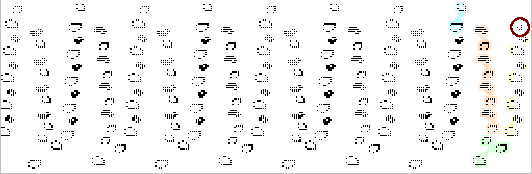
\includegraphics[width=\textwidth]{self_support_spaceships/caterpillar_helix.pdf}}
\caption{A $102c/270 = 17c/45$ helix that is used by the caterpillar spaceship. Four of the glider-shifting flotillae (highlighted in \bgbox{yellowback2}{yellow}) move the glider south, the flotilla highlighted in \bgbox{greenpastel}{green} reflects it and produces an extra glider to the southeast, four more of the glider-shifting flotillae (highlighted in \bgbox{orangeback2}{orange}) move the glider back north, and then the flotilla highlighted in \bgbox{aquaback}{aqua} reflects it back to the south. This sequence of 21 xWSSes then repeats indefinitely.}\label{fig:caterpillar_helix}
\end{figure}

This helix thus travels at a speed of
\[
	\frac{(20m + 20)c}{40m + n + 101}.
\]
To create such a helix with speed $(p/q)c$, where $p$ and $q$ are arbitrary positive integers with $p/q < 1/2$, we can simply choose
\begin{align}\label{eq:orth_helix_parameters}
	m = 4p - 1 \qquad \text{and} \qquad n = 80(q - 2p) - 61.
\end{align}
The fact that $m$ is a non-negative integer is clear, and $n$ being a non-negative integer follows from the fact that $p/q < 1/2$, so $q - 2p \geq 1$.\footnote{The inequality $p/q < 1/2$ is equivalent to $q - 2p > 0$. To get the (seemingly) stronger inequality $q - 2p \geq 1$, recall that $p$ and $q$ are integers.} Some mildly ugly algebra also reveals that
\begin{align*}
	\frac{20m + 20}{40m + n + 101} & = \frac{20(4p - 1) + 20}{40(4p - 1) + (80(q - 2p) - 61) + 101} \\
	& = \frac{80p - 20 + 20}{160p - 40 + 80q - 160p - 61 + 101} = \frac{80p}{80q} = \frac{p}{q},
\end{align*}
as desired. For emphasis, we state what we have just demonstrated as a theorem:

\begin{theorem}[Universality of Orthogonal Helices]\label{thm:universality_orthogonal_helices}
	The three reactions from Figure~\ref{fig:helix_operations} can be used to create an orthogonal helix, which fires gliders forward on one side, with any rational speed slower than $c/2$.
\end{theorem}

It is worth noting that the values of $m$ and $n$ given by Equation~\eqref{eq:orth_helix_parameters} are typically much larger than necessary---we chose those \emph{formulas} for $m$ and $n$ to be simple, but much smaller \emph{values} of $m$ and $n$ can typically be found. For example, if $p = 17$ and $q = 45$ then those formulas give $m = 67$ and $n = 819$, which would result in a monstrously large helix consisting of $273$ xWSSes. However, the smaller values $m = 16$ and $n = 159$ give a helix of the same speed consisting of ``only`` $69$ xWSSes.

To decrease these values even further, simply notice that we can add\footnote{Or subtract---some uninterrupted travel time can be removed from the output gliders in the reactions from Figures~\ref{fig:helix_reflect} and~\ref{fig:helix_duplicate}.} some uninterrupted glider travel time to the helix. If we let the glider travel, unaffected by xWSSes, for $\ell$ additional cells in each direction of the helix, then the helix's displacement is increased by $2\ell$~cells, while its period is increased by $4(2\ell) = 8\ell$~generations. The speed of this new helix would then be
\[
	\frac{(20m + 2\ell + 20)c}{40m + 8\ell + n + 101},
\]
and strategic choices of $\ell$ can lead to smaller helices. For example, picking $\ell = 1$, $m = 4$, and $n = 1$ gives us exactly the $17c/45$ helix from Figure~\ref{fig:caterpillar_helix} that consists of $21$~xWSSes.


\subsection{The Caterpillar Itself}\label{sec:caterpillar_itself}

Putting all of these ideas together finally gives us the caterpillar spaceship,\footnote{The components used in the caterpillar were found by Gabriel Nivasch, David Bell, and Jason Summers, and construction was completed in December 2004 by a computer program written by Nivasch (see \httpurl{gabrielnivasch.org/fun/life/caterpillar}).} displayed in Figure~\ref{fig:caterpillar}, which has a very similar shape and basic structure to that of the silverfish. However, it is absolutely gargantuan, even compared to the silverfish---it is over $7$ times as long and has over $50$ times as many live cells. The primary reason for this drastic increase in size is that it has to synthesize the $21$-xWSS helix from Figure~\ref{fig:caterpillar_helix} on its side, whereas the silverfish just needed to synthesize the $2$-HWSS flotilla from Figure~\ref{fig:g_2h_to_m}.

\begin{figure}[!htbp]
	\centering
	\embedlink{caterpillar}{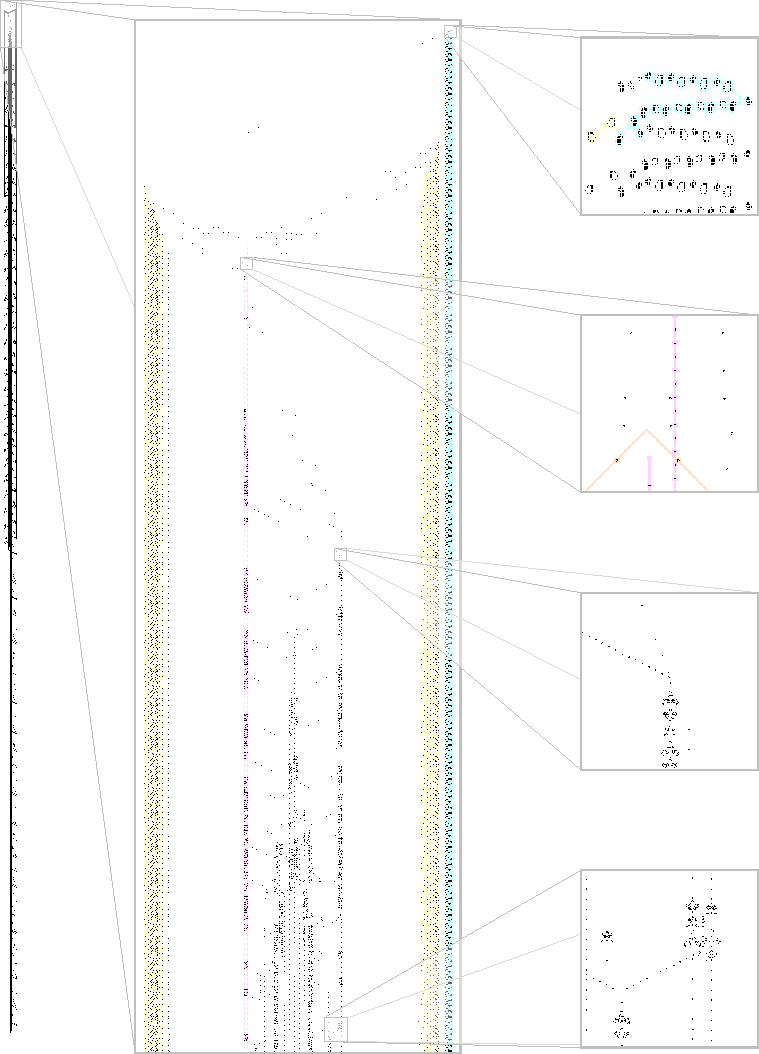
\includegraphics[width=\textwidth]{self_support_spaceships/caterpillar.pdf}}
	\caption{The $17c/45$ orthogonal \textbf{caterpillar} spaceship, travelling up. The helix along its right side (highlighted in \bgbox{aquaback}{aqua}) periodically fires a glider that hits numerous glider duplicators (highlighted in \bgbox{yellowback2}{yellow}) so as to synthesize the frontmost pair of blinker tracks (highlighted in \bgbox{magentaback}{magenta}). Those two blinker tracks then synthesize $38$ more blinker tracks so that numerous pi-crawler rakes can travel on them and synthesize the afore-mentioned helix and glider duplicators.}\label{fig:caterpillar}
\end{figure}

Actually, it's worse than this---because the caterpillar's helix has period $102 = 6 \times 17$, it seems like we should need $24$ copies of this helix ($6$ on each side for each of the $2$ blinker tracks that they need to synthesize). However, the caterpillar uses some glider-duplication tricks so that it ``only'' needs an extra 30 or so xWSSes on each side (see Exercise~\ref{exer:caterpillar_glider_duplicate}). To synthesize this extreme number of xWSSes on its sides a bit more efficiently, the caterpillar uses several columns of rakes on parallel tracks to implement non-slow synthesis, whereas the silverfish used just a single column of rakes down its center to implement slow salvo synthesis.\footnote{Also, slow salvo synthesis was not as fully developed when the caterpillar was constructed, so non-slow synthesis was the only realistic option at the time.}


%%%%%%%%%%%%%%%%%%%%%%%%%%%%%%%%
\section{Oblique Helices and the Waterbear}\label{sec:waterbear}\index{waterbear}
%%%%%%%%%%%%%%%%%%%%%%%%%%%%%%%%

Another self-supporting spaceship that works in much the same way as the silverfish and caterpillar is the \textbf{waterbear}. The reaction\index{(23,5)/79 reaction} at the heart of this spaceship is displayed in Figure~\ref{fig:23_5c_79_reaction}, and consists of a Herschel colliding with a glider so as to displace itself by $(23,5)$ over the course of $79$ generations while duplicating the glider.

\begin{figure}[!htb]
	\centering
	\patternimglink{0.0768}{23_5c_79_reaction}
	\caption{The \textbf{(23,5)c/79 reaction}, in which a Herschel (displayed in \bgbox{greenpastel}{green}) moves obliquely along a glider track while duplicating that track. The cells displayed in \bgbox{redback}{red} simply die off in two more generations.}\label{fig:23_5c_79_reaction}
\end{figure}

Much like the $31c/240$ reaction from Figure~\ref{fig:31c_240_reaction} and the $17c/45$ reaction from Figure~\ref{fig:reburnable_blinker_wick}, this $(23,5)c/79$ reaction is a prime candidate for the central spine of a self-supporting spaceship. We ``just'' need to find a way to use its output gliders to synthesize the necessary input gliders from the front. We do not explore most of the techniques that make this possible. However, we do note that, since this reaction moves faster than a glider (i.e., $c/4$), we again need to use the backward gliders to synthesize a helix that travels to the front of the spaceship.

Constructing a helix that travels at the correct speed might seem problematic, since xWSSes all move orthogonally, whereas we need the helix to move obliquely at $(23,5)c/79$. Remarkably, this is not actually a problem---the exact same reactions that we used in Section~\ref{sec:caterpillar_helices} to create orthogonal helices can in fact be used to create \emph{oblique} helices that travel at the same speed and angle as any spaceship.\footnote{We know from Exercise~\ref{exer:general_speed_limit} that a spaceship that displaces itself by $(x,y)$ over the course of its period must have speed no larger than $(x,y)c/(2x+2y)$.}

\begin{theorem}[Universality of Oblique Helices]\label{thm:universality_oblique_helices}
	For any integers $x \geq y > 0$, the three reactions from Figure~\ref{fig:helix_operations} can be used to create an oblique helix, which fires gliders forward on one side, with any rational speed that is no faster than $(x,y)c/(2x + 2y)$. In particular, such helices exist that travel at the same speed and direction as any oblique spaceship.
\end{theorem}

Indeed, the only modification that we have to make to our orthogonal method of constructing helices is to use fewer glider-shifting flotillae on one half of the helix than on the other. For example, the helix displayed in Figure~\ref{fig:50_13c_161_helix} uses two copies of that flotilla in one direction, but only one copy of it in the other, and ends up travelling obliquely at a speed of $(50,13)c/161$.

\begin{figure}[!htb]
	\centering
	\embedlink{50_13c_161_helix}{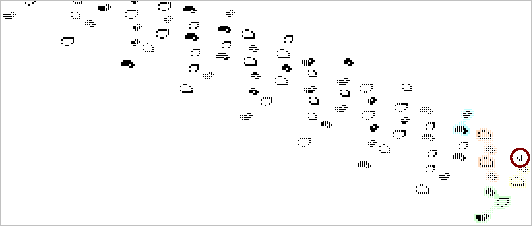
\includegraphics[width=\textwidth]{self_support_spaceships/50_13c_161_helix.pdf}}
	\caption{A $(50,13)c/161$ helix that is oblique since it uses fewer of the glider-shifting flotillae to move the glider south (highlighted in \bgbox{yellowback2}{yellow}) than it does to move the glider back north (highlighted in \bgbox{orangeback2}{orange}).}\label{fig:50_13c_161_helix}
\end{figure}

We should also note that, for oblique helices, there are two different ``forward'' directions (and two different ``backward'' directions) that a glider can be fired in. That direction it determined by which side of the helix has the glider-duplicating flotilla on it. For example, interchanging the green and aqua flotillae in Figure~\ref{fig:50_13c_161_helix} results in a helix that travels at the same speed and slope, but fires forward gliders at a different angle.

\begin{proof}[Proof of Theorem~\ref{thm:universality_oblique_helices}.]
	We proceed mostly as in the proof of the corresponding result for orthogonal helices (Theorem~\ref{thm:universality_orthogonal_helices})---the main difference is that instead of using $m$ of the glider-shifting flotillae in each direction of the helix, we use $k$ of them in one direction and $m$ of them in the other (so, for example, $k = 2$ and $m = 1$ in the oblique helix from Figure~\ref{fig:50_13c_161_helix}). This helix travels at a speed of
	\begin{align}\label{eq:oblique_speed_helix}
		\frac{(10k + 10m + 20, 13k - 13m)c}{20k + 20m + n + 101},
	\end{align}
	where $n$ is again the number of generations that the final xWSS pair is delayed in the glider duplicator from Figure~\ref{fig:helix_duplicate}.\footnote{For example, if $k = 2$, $m = 1$, and $n = 0$ then we get a helix with speed $(20 + 10 + 20, 26 - 13)c/(40 + 20 + 101) = (50,13)c/161$, as in Figure~\ref{fig:50_13c_161_helix}.}
	
	To create such a helix with speed $(x,y)c/q$, where $x$, $y$, and $q$ are arbitrary positive integers with $y/q \leq x/q < 1/2$,\footnote{This is actually a stronger result than in the statement of the theorem. These helices can travel diagonally at speeds arbitrarily close to $c/2$, for example, despite the $c/4$ diagonal spaceship speed limit. The reason that this does not contradict Theorem~\ref{thm:speed_limits} is that the glider is not travelling through empty space---it is burning through xWSSes.} we can simply choose
	\begin{align*}
		k = 13x + 10y - 1, \qquad m = 13x - 10y - 1, \qquad \text{and} \qquad n = 260(q - 2x) - 61.
	\end{align*}

	The fact that $k$ is a non-negative integer is clear, $m$ being a non-negative integer follows from the fact that $x \geq y \geq 1$, so $m = 13x - 10y - 1 \geq 3x - 1 \geq 2$, and $n$ being a positive integer follows from the fact that $x/q < 1/2$ implies $q - 2x \geq 1$. Finally, direct (and more-than-mildly ugly) calculation reveals that
	\begin{align*}
		& \frac{(10k + 10m + 20, 13k - 13m)c}{20k + 20m + n + 101} \\
		& \qquad = \frac{\big(10(13x + 10y - 1) + 10(13x - 10y - 1) + 20, 13(13x + 10y - 1) - 13(13x - 10y - 1)\big)c}{20(13x + 10y - 1) + 20(13x - 10y - 1) + (260(q - 2x) - 61) + 101} \\
		& \qquad = \frac{(130x + 100y - 10 + 130x - 100y - 10 + 20, 169x + 130y - 13 - 169x + 130y + 13)c}{260x + 200y - 20 + 260x - 200y - 20 + 260q - 520x - 61 + 101} \\
		& \qquad = \frac{(260x, 260y)c}{260q} = \frac{(x,y)c}{q},
	\end{align*}
	as desired.
\end{proof}

The waterbear's helix makes use of slightly different components than the ones we introduced for use in the caterpillar (see Exercise~\ref{exer:waterbear_one_more_helix_component} and Figure~\ref{fig:waterbear}), so as to reduce its size down to just $6$ xWSSes, and also so that it fires gliders backwards instead of forwards.\footnote{Again, for oblique helices there are two different ``backwards'' directions that gliders can be fired in.} Fortunately, we can construct backwards-firing helices that travel at any speed and slope, just as we could with forwards-firing helices (see Exercise~\ref{exer:backward_helix_universal}).

\begin{figure}[!htbp]
	\centering
	\embedlink{waterbear}{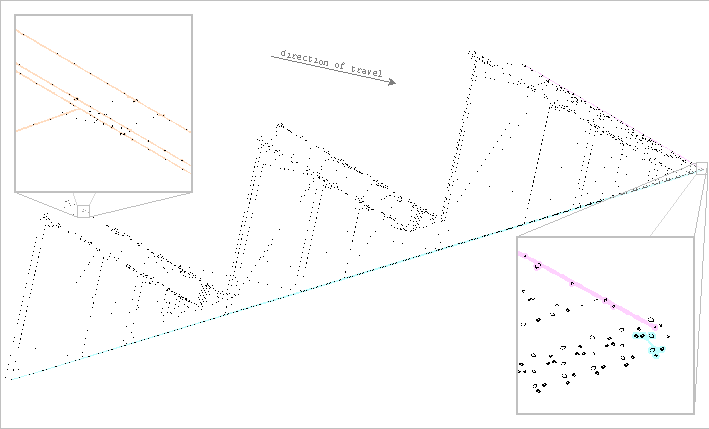
\includegraphics[width=\textwidth]{self_support_spaceships/waterbear.pdf}}
	\caption{The $(23,5)c/79$ oblique \textbf{waterbear} spaceship. The helix along its southeast side (highlighted in \bgbox{aquaback}{aqua}) periodically fires a backward glider that supports a Herschel via the $(23,5)c/79$ reaction on its northeast side (highlighted in \bgbox{magentaback}{magenta}). The output gliders from that reaction are then used to synthesize additional tracks and the afore-mentioned helix. Constructed by Brett Berger in December 2014, based on numerous reactions (such as the helix) that were found by Ivan Fomichev.}\label{fig:waterbear}
\end{figure}

Unlike the caterpillar, in which the primary $17c/45$ reaction moved parallel to the helix, the waterbear's $(23,5)c/79$ reaction runs at a different angle than the helix. The result of this change is that, instead of being long and thin like the caterpillar, the simplest waterbear to construct is triangular, with the helix along one side of the triangle and the $(23,5)c/79$ reaction along another. To keep its size down a bit, the $(23,5)/79$ Herschel-and-glider track on one of the sides is ``reset'' at two points, so that the resulting waterbear looks like it is made up of $3$ much smaller triangles instead. As a result, it has $197{\thousep}896$ live cells and fits in a $13{\thousep}295 \times 28{\thousep}010$ bounding box, making it comparable in size to the silverfish.



%%%%%%%%%%%%%%%%%%%%%%%%%%%%%%%%
\section{Caterloopillars}\label{sec:caterloopillar}\index{caterloopillar}
%%%%%%%%%%%%%%%%%%%%%%%%%%%%%%%%

The final family of self-supporting spaceships that we look at are called \textbf{caterloopillars}. The basic idea behind these spaceships is the same as it was for the silverfish, caterpillar, and waterbear: many copies of a central moving reaction are used to produce gliders that collaborate so as to send signals forward and build their own support structures ahead of themselves. However, we now flip this idea on its head---what if instead of using an infinite trail of stable objects like blocks or blinkers to support a naturally-moving object like a Herschel or pi-heptomino, we use an infinite trail of spaceships to move a stable object?\footnote{This basic idea for the construction of a caterloopillar spaceship was originally proposed by David Bell in October 2006. It wasn't until April 2016 that slow-salvo technology had advanced to the point that it was actually constructed.}


\subsection{Loaf Tracks}\label{sec:caterloopillar_loaf_track}

For a still-life-moving reaction to actually be usable at the core of a self-supporting spaceship, it also needs to produce some sort of output (ideally a glider) that can then be used to synthesize the spaceships that pull the stable object. One such reaction, which uses three xWSS flotillae to push a loaf forward while also generating a glider, is displayed in Figure~\ref{fig:caterloopillar_loaf_pusher}.\footnote{In contrast with the glider-manipulating flotillae that are used in helices (refer back to Section~\ref{sec:caterpillar_helices}), these flotillae are \emph{not} destroyed by the glider.}

\begin{figure}[!htb]
	\centering
	\embedlink{caterloopillar_loaf_pusher}{\vcenteredhbox{\phantom{\genarrow{224}}} \vcenteredhbox{
\includegraphics[width=0.918\textwidth]{self_support_spaceships/caterloopillar_loaf_mover_0.pdf}}} \\[1em]
	
	\patternlink{caterloopillar_loaf_pusher}{\vcenteredhbox{\genarrow{224}} \vcenteredhbox{
\includegraphics[width=0.918\textwidth]{self_support_spaceships/caterloopillar_loaf_mover_224.pdf}}} \\[1em]
	
	\patternlink{caterloopillar_loaf_pusher}{\vcenteredhbox{\genarrow{164}} \vcenteredhbox{
\includegraphics[width=0.918\textwidth]{self_support_spaceships/caterloopillar_loaf_mover_388.pdf}}} \\[1em]
	
	\patternlink{caterloopillar_loaf_pusher}{\vcenteredhbox{${} \, {}$ \genarrow{64}} \vcenteredhbox{
\includegraphics[width=0.918\textwidth]{self_support_spaceships/caterloopillar_loaf_mover_452.pdf}}}
	
	\caption{An arrangement of three xWSS flotillae that push a loaf forward by $46$~cells and simultaneously create a glider. The first $4$-xWSS flotilla (highlighted in \bgbox{magentaback}{magenta}) turns the loaf into a glider, the next $3$-MWSS flotilla (highlighted in \bgbox{aquaback}{aqua}) reflects that glider, and finally the $2$-xWSS flotilla (highlighted in \bgbox{greenpastel}{green}) creates a loaf from that glider (without destroying it). Moving the aqua flotilla northwest by $n$~cells and the green flotilla west by $2n$~cells results in the loaf being pushed forward by $46 + 2n$~cells.}\label{fig:caterloopillar_loaf_pusher}
\end{figure}

We will thus use a track of loaves as the central spine of a self-supporting spaceship, with this 9-xWSS flotilla being used to push it forward. As the flotilla pushes the loaves, it also releases gliders that can be used to synthesize supporting mechanisms via unidirectional slow salvo synthesis (in almost exactly the same way as the silverfish used unidirectional slow salvo synthesis to synthesize two HWSSes on each side).

Perhaps the simplest supporting mechanism to synthesize is an xWSS flotilla travelling in the opposite direction that \emph{pulls} a second loaf track by the same amount that the first loaf track is \emph{pushed}. By arranging these two flotillae so that they run on parallel tracks in opposite directions, we can have the loaf-pulling and loaf-pulling flotillae synthesize each other, as illustrated in Figure~\ref{fig:caterloopillar_schematic}.\footnote{The fact that these two flotillae synthesize each other is what gives caterloopillars their name (besides the obvious analogy with the caterpillar)---the xWSSes form a long loop that seems to be synthesizing itself. The name is also a reference to the term ``strange loop'', a concept explored in Douglas Hofstadter's famous book \emph{G\"{o}del, Escher, Bach}.}\index{strange loop}

\begin{figure}[!htbp]
	\centering
	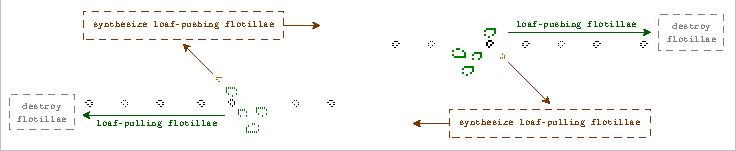
\includegraphics[width=\textwidth]{self_support_spaceships/caterloopillar_schematic.pdf}
	\caption{A schematic for a caterloopillar spaceship that travels to the right. Some loaf-pushing flotillae travel along a loaf track that encodes a unidirectional slow-salvo synthesis of a loaf-pulling flotilla. Those loaf-pulling flotillae travel backwards along a parallel loaf track that encodes a unidirectional slow-salvo synthesis of the loaf-pushing flotilla.}\label{fig:caterloopillar_schematic}
\end{figure}

We just have three tasks that remain in order to actually construct a caterloopillar spaceship with this shape:\smallskip

\begin{itemize}
	\item[1)] Build the loaf-pulling xWSS flotilla.\smallskip
	
	\item[2)] Build mechanisms for destroying the flotillae at the front and back of the spaceship.\smallskip
	
	\item[3)] Come up with unidirectional slow salvo syntheses for these flotillae, and encode them in the spacing between loaves.\smallskip
\end{itemize}

We tackle these three issues one at a time. For (1), we proceed much like we did with the loaf-pushing flotilla that we saw in Figure~\ref{fig:caterloopillar_loaf_pusher}: a loaf-\emph{pulling} flotilla can be built out of smaller flotillae that turn the loaf into a glider, and then rebuild the loaf while duplicating the glider. The particular loaf-pushing flotilla that we used is displayed in Figure~\ref{fig:caterloopillar_loaf_puller}.

\begin{figure}[!htb]
	\centering
	\embedlink{caterloopillar_loaf_puller}{\vcenteredhbox{\phantom{\genarrow{224}}} \vcenteredhbox{
\includegraphics[width=0.918\textwidth]{self_support_spaceships/caterloopillar_loaf_puller_0.pdf}}} \\[1em]
	
	\patternlink{caterloopillar_loaf_puller}{\vcenteredhbox{\genarrow{156}} \vcenteredhbox{
\includegraphics[width=0.918\textwidth]{self_support_spaceships/caterloopillar_loaf_puller_156.pdf}}} \\[1em]
	
	\patternlink{caterloopillar_loaf_puller}{\vcenteredhbox{\genarrow{232}} \vcenteredhbox{
\includegraphics[width=0.918\textwidth]{self_support_spaceships/caterloopillar_loaf_puller_388.pdf}}} \\[1em]
	
	\patternlink{caterloopillar_loaf_puller}{\vcenteredhbox{${} \ \ {}$ \genarrow{8}} \vcenteredhbox{
\includegraphics[width=0.918\textwidth]{self_support_spaceships/caterloopillar_loaf_puller_396.pdf}}}
	
	\caption{An arrangement of three xWSS flotillae that pull a loaf backward by $54$~cells and simultaneously create a glider. The first $4$-xWSS flotilla (highlighted in \bgbox{magentaback}{magenta}) turns the loaf into a pair of gliders, the next $3$-LWSS flotilla (highlighted in \bgbox{aquaback}{aqua}) reflects one of those gliders, and the final LWSS (highlighted in \bgbox{greenpastel}{green}) turns that glider back into a loaf. Moving the aqua flotilla south by $n$~cells and west by $3n$~cells, and the green flotilla west by $6n$~cells, results in the loaf being pulled backward by $54 + 2n$~cells.}\label{fig:caterloopillar_loaf_puller}
\end{figure}

While this reaction does not pull the loaf by the same number of cells that the reaction from Figure~\ref{fig:caterloopillar_loaf_pusher} pushes it, the spacing between the component flotillae that make up these reactions can easily be adjusted so as to fix this problem. In particular, for every integers $m,n \geq 0$, we can adjust the loaf-pushing and loaf-pulling flotillae to move the loaf by $46 + 2m$ and $54 + 2n$ cells, respectively. Choosing $m = n + 4$ results in both flotillae moving the loaf track by $54 + 2n$ cells.


\subsection{The Front and Back Ends}\label{sec:caterloopillar_front_and_back}

To take care of task (2) above---destroying the xWSS flotillae after they are done pushing and pulling the loaf tracks---we can place a constellation of still lifes at the ends of the tracks. The tricky part is moving that constellation down the track at the same speed as the loaves.

To solve this problem, we instead use a \emph{single} still life along with additional xWSS flotillae. Those extra flotillae are arranged so as to convert the still life into a glider that then (a) reconstructs a copy of that single still life farther down the track, and (b) builds a constellation of still lifes that destroys the loaf-moving flotillae. A bit more specifically, we use additional xWSS flotillae that transform the still life as follows:

\noindent\begin{center}
	\centering
	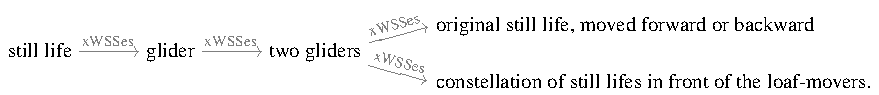
\includegraphics[scale=1]{self_support_spaceships/caterloopillar_front_back_idea.pdf}
\end{center}

Unlike the loaf-moving flotillae, we need the xWSSes in these flotillae to be destroyed as they manipulate the still life and gliders. However, this does not make it any harder to find flotillae that get the job done (in fact, we already saw many one-time glider manipulating flotillae like this when we investigated helices in Section~\ref{sec:caterpillar_helices}). Particular flotillae that can be used at the front and back of the caterloopillar, to destroy the loaf-pusher and loaf-puller that we have already seen, are displayed in Figure~\ref{fig:caterloopillar_front_back}.\footnote{The flotilla from Figure~\ref{fig:caterloopillar_front_end} that destroys the loaf-pusher also releases a backwards glider---see Exercise~\ref{exer:caterloopillar_front_end_glider}.}

\begin{figure}[!htb]
	\centering
	\begin{subfigure}[b]{\textwidth}
		\centering
		\patternimglink{0.0995}{caterloopillar_front_end}
		\caption{A honey farm and 9-xWSS flotilla that can be placed in front of the loaf-pushing flotilla from Figure~\ref{fig:caterloopillar_loaf_pusher} (highlighted in \bgbox{aquaback}{aqua}) so as to destroy it. With the spacing displayed here, the loaf and honeyfarm are each pushed forward by $62$ cells. To increase that displacement to $62 + 2n$ cells, move the top-center MWSS (highlighted in \bgbox{greenpastel}{green}) west by $2n$~cells, the next five xWSSes (highlighted in \bgbox{magentaback}{magenta}) southwest by $n$~cells, and the next two MWSSes (highlighted in \bgbox{yellowback2}{yellow}) and loaf-pusher southwest by $2n$~cells.}\label{fig:caterloopillar_front_end}
	\end{subfigure}\\[0.3cm]
	\begin{subfigure}[b]{\textwidth}
		\centering
		\patternimglink{0.066}{caterloopillar_back_end}
		\caption{A beehive and 10-xWSS flotilla that can be placed in front of the loaf-pulling flotilla from Figure~\ref{fig:caterloopillar_loaf_puller} (highlighted in \bgbox{aquaback}{aqua}) so as to destroy it. With the spacing displayed here, the loaf and beehive are each pulled backward by $94$ cells. To increase that displacement to $94 + 2n$ cells, move the bottom-center MWSS (highlighted in \bgbox{greenpastel}{green}) west by $6n$~cells, the next five xWSSes (highlighted in \bgbox{magentaback}{magenta}) north by $n$~cells and west by $3n$~cells, and the next three xWSSes (highlighted in \bgbox{yellowback2}{yellow}) and loaf-pusher north by $2n$~cells and west by $4n$~cells.}\label{fig:caterloopillar_back_end}
	\end{subfigure}
	\caption{Some xWSS flotillae and still lifes that can be placed in front of the loaf-moving flotillae so as to destroy them. When adjusting these flotillae, also adjust the loaf-pushing and loaf-pulling flotillae as indicated in the captions of Figures~\ref{fig:caterloopillar_loaf_pusher} and~\ref{fig:caterloopillar_loaf_puller}, respectively.}\label{fig:caterloopillar_front_back}
\end{figure}


\subsection{Putting It All Together}\label{sec:caterloopillar_itself}

All that is left now to complete the caterloopillar is task (3)---coming up with a unidirectional slow-salvo glider synthesis of the xWSS flotillae from Figure~\ref{fig:caterloopillar_front_back} that will travel antiparallel to each other. In fact, we even need this glider synthesis to be \textbf{monochromatic}---consisting entirely of gliders of just one color.\index{monochromatic} Indeed, the locations from which gliders are fired is determined by the spacing of the loaves on the loaf track, and that spacing is orthogonal (i.e., the loaves and hence gliders in the slow salvo are separated by full diagonals, not half diagonals).

Such a glider synthesis will consist of hundreds of steps, so actually coming up with it is best left to a computer script.\footnote{Such a script, which was made by Michael Simkin and used to construct the first caterloopillars in April 2016, is available at \httpsurl{conwaylife.com/forums/viewtopic.php?p=30104\#p30089}.} Once we have that glider synthesis, though, we are done, and get a completed caterloopillar like the one displayed in Figure~\ref{fig:caterloopillar}.

\begin{figure}[!htbp]
	\centering
	\embedlink{caterloopillar}{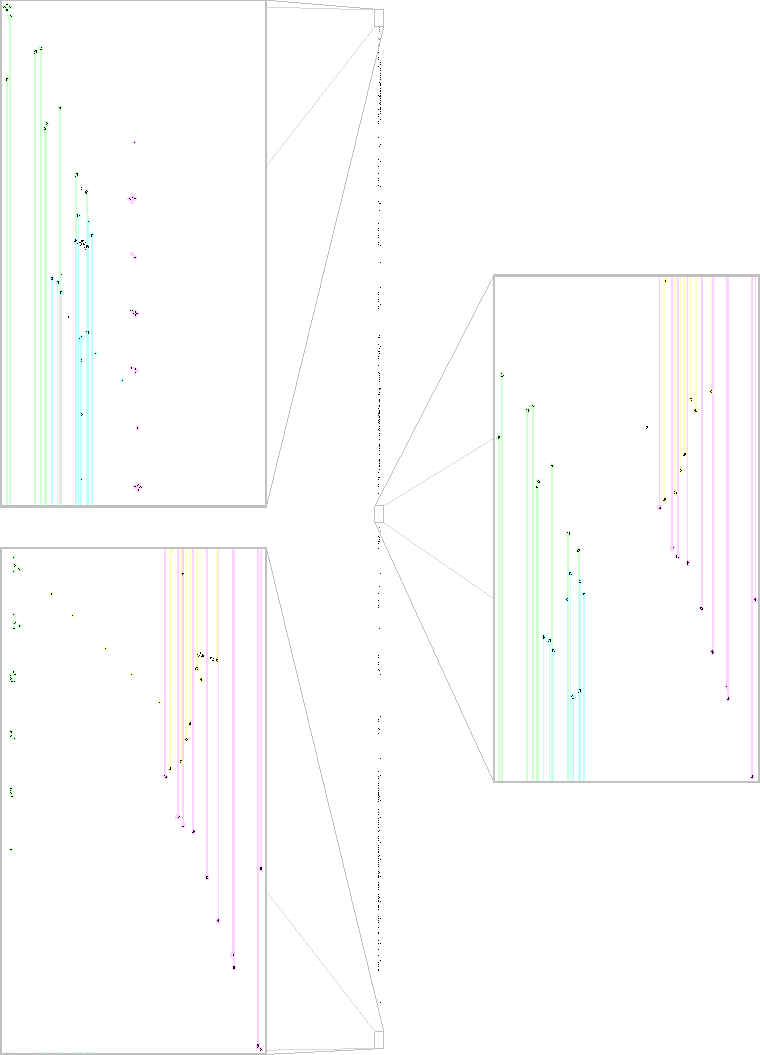
\includegraphics[width=\textwidth]{self_support_spaceships/caterloopillar.pdf}}
	\caption{A $c/24$ orthogonal \textbf{caterloopillar} spaceship, travelling up. At the top, the loaf-pushing flotillae (highlighted in \bgbox{aquaback}{aqua}) and their destroyers (highlighted in \bgbox{greenpastel}{green}) begin synthesizing the loaf-pulling flotillae (highlighted in \bgbox{yellowback2}{yellow}) and their destroyers (highlighted in \bgbox{magentaback}{magenta}). At the bottom, the loaf-pullers begin synthesizing the loaf-pushers. In the middle, these flotillae simply pass by each other.}\label{fig:caterloopillar}
\end{figure}

This particular caterloopillar pushes and pulls the loaf track by $98$~cells per period, and the forward-travelling xWSS flotillae are separated by $1{\thousep}078$~cells, for a speed of $98c/(2(1078 + 98)) = 98c/2352 = c/24$.\footnote{The speed is $98c/(2(1078 + 98))$ instead of just $98c/(2 \cdot 1078)$ because of a ``doppler effect'': the flotillae do not have to travel just $1{\thousep}078$ cells per period, but also the extra $98$ cells that the still lifes were pushed.}\index{doppler effect} Caterloopillars of many other speeds can be straightforwardly created from this one, though. For example, we could straightforwardly (though tediously!) move the flotillae farther apart, resulting in larger caterloopillars that travel much more slowly.

Similarly, we can also squeeze the flotillae closer together, resulting in slightly smaller and faster caterloopillars, but we are much more limited in this direction. For example, the forward flotillae used by this caterloopillar must be separated by at least $352$ cells, so these simple adjustments cannot possibly produce caterloopillars that are any faster than $98c/(2(352 + 98)) = 49c/450$.

To create even faster caterloopillars, we have to increase how far the flotillae from Figure~\ref{fig:caterloopillar_front_back} push and pull their still lifes, which requires us to adjust the slow salvo syntheses that is used to construct those flotillae. We thus have to rebuild the caterloopillar almost entirely from scratch (or, rather, the computer script has to rebuild it from scratch). If we are willing to put in this extra bit of effort, then we can construct caterloopillars that travel at any rational speed slower than $c/4$:\footnote{This $c/4$ speed limit should be fairly intuitive---as we increase the amount that the caterloopillar displaces its still lifes per period, more and more of its travel time is spent as a ($c/4$) glider bouncing between the components of the flotillae from Figure~\ref{fig:caterloopillar_front_back}. Reaching the theoretical speed limit of $c/2$ would require a major redesign.}

\begin{theorem}[Caterloopillar Speeds]\label{thm:caterloopillar_speeds}
	Caterloopillar spaceships can be constructed that travel at any rational speed slower than $c/4$.
\end{theorem}

\begin{proof}
	For any integers $m,n \geq 0$, if the flotilla from Figure~\ref{fig:caterloopillar_front_end} is configured to push the loaf and honey farm forward by $100 + 2n$ cells, then we can separate subsequent copies of this flotilla by $400 + 2n + 2m$ cells.\footnote{That is, we can separate copies of these flotillae by any even number of cells that is at least as large as $400 + 2n$. Even though the width of that flotillae is actually $682 + 4n$ cells, they can ``overlap'' considerably, with one copy of the loaf pusher being nestled underneath the previous loaf-pusher-destroyer.} Similarly, if the flotilla from Figure~\ref{fig:caterloopillar_back_end} is configured to pull the loaf and beehive backward by $100 + 2n$ cells, then we can separate separate copies of it by $600 + 6n + 2m$ cells.
	
	It follows that the speed of the resulting caterloopillar is
	\[
		\frac{(100 + 2n)c}{2\big((400 + 2n + 2m) + (100 + 2n)\big)} = \frac{(50 + n)c}{500 + 4n + 2m}.\footnote{We calculated this speed based on the loaf-pulling flotillae. If we instead calculated it based on the loaf-\emph{pulling} flotillae, we would get the same answer: $(100 + 2n)c/\big(2((600 + 6n + 2m) - (100 + 2n))\big) = (50 + n)c/(500 + 4n + 2m)$.}
	\]
	
	To create a caterloopillar with speed $(p/q)c$, where $p,q > 0$ are integers with $p/q < 1/4$, it suffices to choose
	\[
		n = 300p - 50 \qquad \text{and} \qquad m = 150(q - 4p) - 150.
	\]
	These are both non-negative integers, and straightforward algebra shows that
	\[
		\frac{50 + n}{500 + 4n + 2m} = \frac{50 + (300p - 50)}{500 + 4(300p - 50) + 2(150(q - 4p) - 150)} = \frac{300p}{300q} = \frac{p}{q},
	\]
	as claimed.
\end{proof}

It is worth noting that faster caterloopillars are typically larger than slower ones, not just because their component flotillae become more spaced out, but also because the glider syntheses used to construct those flotillae require more steps. \emph{Roughly} the same synthesis recipes can be used in all caterloopillars, but additional seed-moving steps are required if the xWSSes that make up the loaf-moving flotillae are separated by large distances.

Because of some ugliness involving these unidirectional slow-salvo glider syntheses, caterloopillars have only been explicitly constructed for speeds of the form $(p/q)c$ (where $p/q$ is in lowest terms and $p/q < 1/4$) when $q \not\equiv 2 \pmod{4}$. For example, no one has constructed a caterloopillar with speed $c/18$ or $5c/18$, but caterloopillars have been constructed with speeds $c/15$, $c/16$, $c/17$, and $2c/18 = c/9$. Regardless of this limitation, caterloopillars of these troublesome speeds still \emph{exist}, thanks to Theorem~\ref{thm:caterloopillar_speeds}.

The fastest caterloopillar that has been explicitly constructed so far has speed $19c/80$. It is approximately $10$ times as long and wide as the $c/24$ caterloopillar from Figure~\ref{fig:caterloopillar}, and also has about $10$ times as many live cells.


%%%%%%%%%%%%%%%%%%%%%%%%%%%%%%%%
\section{Notes and Historical Remarks}\label{sec:self_support_history}
%%%%%%%%%%%%%%%%%%%%%%%%%%%%%%%%

Despite its monstrous size, the silverfish displayed in Figure~\ref{fig:silverfish} is currently the smallest $31c/240$ orthogonal spaceship known in Life. About six years prior to its construction, two other spaceships of this same speed were built using most of the same reactions. These spaceships, called the \textbf{shield bug}\index{shield bug} and the \textbf{centipede},\index{centipede} are displayed in Figure~\ref{fig:centipede_shield_bug}. They were completed on the same day---September 4, 2014---by Dave Greene and Chris Cain, respectively, with help from Kiho Park, Ivan Fomichev and Adam P.~Goucher.

\begin{figure}[!htbp]
	\centering
	\begin{tabular}{@{}cc@{}}
		\begin{subfigure}{0.5333\textwidth}
			\embedlink{shield_bug}{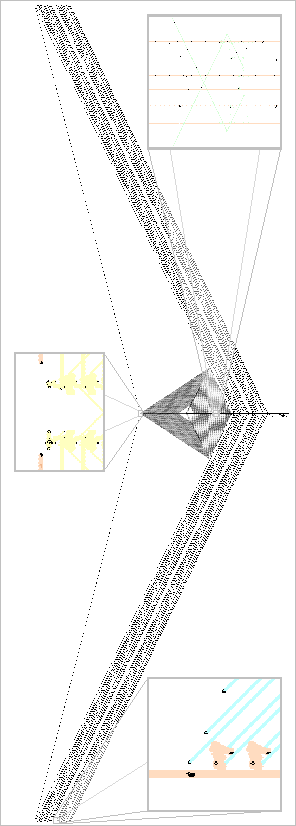
\includegraphics[width=\textwidth]{self_support_spaceships/shield_bug.pdf}}
			\caption{The \textbf{shield bug}, travelling to the left.}\label{fig:shield_bug}
		\end{subfigure} &
		\begin{subfigure}{0.4267\textwidth}
			\centering
			\embedlink{centipede}{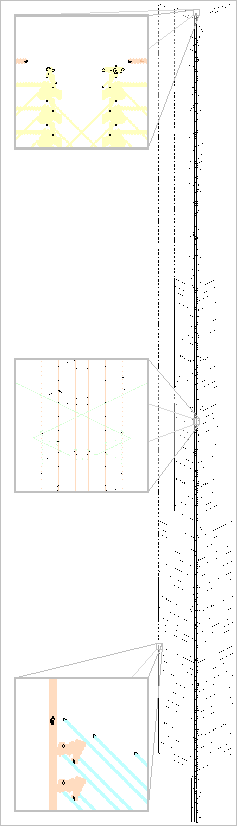
\includegraphics[width=\textwidth]{self_support_spaceships/centipede.pdf}}
			\caption{The \textbf{centipede}, travelling up.}\label{fig:centipede}
		\end{subfigure}
	\end{tabular}
	\caption{A pair of (huge) $31c/240$ spaceships based on the same Herschel-crawling reaction as the silverfish. They each use six-block tracks that carry Herschel-based rakes down their center, and the same double-HWSS slow salvo synthesis on their sides to stabilize the front end.}
	\label{fig:centipede_shield_bug}
\end{figure}

When measuring size according to number of live cells, these spaceships are roughly $16$ and $3$ times as large as the silverfish, respectively. The reason that the silverfish could be so much smaller is that it uses a new front end (which was found by Chris Cain just 16 days after he completed the centipede) that is supported by just two heavyweight spaceships on each side instead of six.

Besides the $31c/240$, $17c/45$, and $(23,5)c/79$ reactions that we saw in this chapter, there are numerous other known reactions that involve an object moving through a stable or glider-based wick---such reactions are called \textbf{crawlers}\index{crawler} or \textbf{climbers}).\index{climber|see {crawler}} Four such crawlers are displayed in Figure~\ref{fig:self_support_climbers}, and each one of them could potentially be used to construct a self-supporting spaceship using the same techniques from this chapter.

\begin{figure}[!htb]
	\centering
	\begin{subfigure}{0.495\textwidth}
		\centering
		\patternimglink{0.103}{13_1c_31_b_heptomino_climber}
		\caption{A $(13,1)c/31$ B-heptomino crawler.}\label{fig:13_1c_31_b_heptomino_climber}
	\end{subfigure} \ \ \ \begin{subfigure}{0.475\textwidth}
	 	\centering
	 	\patternimglink{0.07891384615}{27_1c_72_herschel_climber}
	 	\caption{A $(27,1)c/72$ Herschel-pair crawler.}\label{fig:27_1c_72_herschel_climber}
	\end{subfigure} \\[0.2cm]
	\begin{subfigure}{0.495\textwidth}
		\centering
		\patternimglink{0.07}{34_7c_156_herschel_climber}
		\caption{A $(34,7)c/156$ Herschel crawler.}\label{fig:34_7c_156_herschel_climber}
	\end{subfigure} \ \ \ \begin{subfigure}{0.475\textwidth}
		\centering
		\patternimglink{0.08439588688}{half_bakery_reaction}
		\caption{A $(3,6)$ half-bakery crawler.}\label{fig:half_bakery_reaction}
	\end{subfigure}
	\caption{Some crawlers that could potentially be used to construct self-supporting spaceships.}\label{fig:self_support_climbers}
\end{figure}
% (13,1)c/31: https://www.conwaylife.com/forums/viewtopic.php?f=2&t=1182
% (27,1)c/72: https://www.conwaylife.com/forums/viewtopic.php?f=2&t=2130
% (34,7)c/156: https://www.conwaylife.com/forums/viewtopic.php?f=2&t=2286

Of these crawlers, the $(3,6)$ half-bakery reaction\index{half-bakery} from Figure~\ref{fig:half_bakery_reaction} is by far the easiest to work with, since a half-bakery is stable and thus the timing of the gliders is almost completely irrelevant. Indeed, this reaction has actually been used to create another self-supporting spaceship (essentially the only self-supporting spaceship other than the ones that we saw earlier in this chapter).

The way it works is based on the fact that two copies of this half-bakery reaction can be placed next to each other so as to produce a perpendicular glider (much like we placed two copies of the pi-crawler next to each other to create output gliders back in Figure~\ref{fig:pi_backward_rake}). We can thus use two gliders on a pair of half-bakery tracks to output sequences of gliders, and by using one more glider on a third parallel half-bakery track, we can reflect those gliders by 180 degrees. If we use even more parallel copies of these reactions (seven in total), we can have the triples of output gliders collide with each other in one of the tee\index{tee} reactions from Table~\ref{tab:3_glider_synth}, as illustrated in Figure~\ref{fig:hbk_reactions}.

\begin{figure}[!htb]
	\centering
	\embedlink{half_baked_knightship_reactions}{\vcenteredhbox{\patternimg{0.093}{hbk_reactions_0}} \vcenteredhbox{\genarrow{299}} \vcenteredhbox{\patternimg{0.093}{hbk_reactions_299}} \vcenteredhbox{\genarrow{259}} \vcenteredhbox{\patternimg{0.093}{hbk_reactions_558}}}
	\caption{Some reactions in which gliders travelling southewest along half-bakery trails generate gliders travelling in any of the three other directions. In the northeast arrangement of half-bakeries (highlighted in \bgbox{magentaback}{magenta}), sparks from the half-bakery crawlers collide with each other so as to generate gliders that then collide in a tee reaction (highlighted in \bgbox{greenpastel}{green}). In the southwest arrangement of half-bakeries (highlighted in \bgbox{yellowback2}{yellow}), the half bakeries are separated a bit more so that their sparks do not interfere with each other, thus producing no gliders.}\label{fig:hbk_reactions}
\end{figure}

These reactions give us the freedom to generate gliders travelling in any direction, and in particular they allow us to send gliders back to the start of the half-bakery trails. Those gliders can then use slow salvo synthesis to recreate the gliders that follow the half-bakery trails. In other words, we can use a handful of gliders travelling along half-bakery trails to implement armless construction (as introduced in Section~\ref{sec:armless}) of that handful of gliders.

Spaceships that use these ideas based on the half-bakery crawler are called \textbf{half-baked knightships},\index{half-baked knightship} and the one displayed in Figure~\ref{fig:parallel_hbk}, which was constructed by Chris Cain in July 2014,\footnote{The first half-baked knightship was built by Adam P.~Goucher just $5$ days earlier, and was roughly $10$ times as long, wide, and populous. Dave Greene and Ivan Fomichev helped come up with some of the component reactions and syntheses used in each of these knightships.} is called the \textbf{parallel half-baked knightship}\index{parallel half-baked knightship} (or \textbf{parallel HBK}\index{parallel HBK|see {parallel half-baked knightship}} for short).

\begin{figure}[!htb]
	\centering
	\embedlink{parallel_hbk}{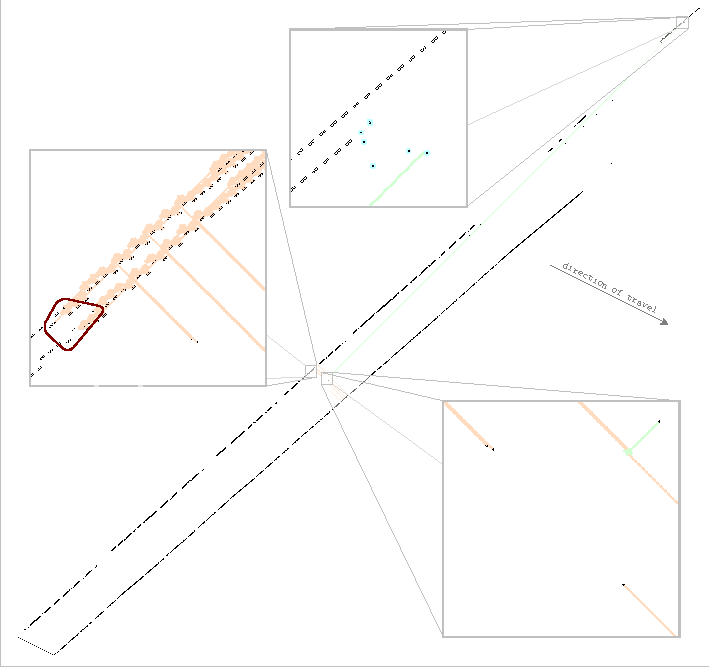
\includegraphics[width=\textwidth]{self_support_spaceships/parallel_hbk.pdf}}
	\caption{The \textbf{parallel half-baked knightship}. Its sides are tracks of half-bakeries that a total of $7$ gliders follow along ($4$ on the northwest tracks, circled in \bgbox{redback}{red}, and $3$ on the southeast tracks). Those gliders move the half-bakeries by $(3,6)$ per period via the half-bakery crawler of Figure~\ref{fig:half_bakery_reaction}, while producing backward-firing gliders via the reactions of Figure~\ref{fig:hbk_reactions} (highlighted in \bgbox{greenpastel}{green}). Those gliders go all the way back to the start of the half-bakery tracks and re-synthesize the original $7$ gliders via a seed highlighted in \bgbox{aquaback}{aqua}.}\label{fig:parallel_hbk}
\end{figure}

The other three crawlers displayed in Figure~\ref{fig:self_support_climbers} have not yet been turned into self-supporting spaceships. One of the main reasons for this is simply that constructing a self-supporting spaceship is a monumental task. However, they are also all slightly more difficult to work with than, for example, the $(23,5)c/79$ reaction from Figure~\ref{fig:23_5c_79_reaction} at the core of the waterbear:\smallskip

\begin{itemize}
	\item The $(13,1)c/31$ B-heptomino crawler from Figure~\ref{fig:13_1c_31_b_heptomino_climber} moves very fast: $13c/31 \approx 0.42c$ in one of the orthogonal directions, which is faster than any self-constructing spaceship that has ever been built as of this writing. As a result, all known helices that travel at this speed and slope are rather large, making any spaceship that would be built from this reaction also rather large (even by self-supporting spaceship standards). For example, any forward-firing helix of this speed and slope that is built out of the components from Figure~\ref{fig:helix_operations} must contain at least 35 xWSSes (see Exercise~\ref{exer:13_1c_31_helix_large}).\smallskip
	
	\item The $(27,1)c/72$ Herschel-pair crawler from Figure~\ref{fig:27_1c_72_herschel_climber} does not produce an extra output glider that can be used to synthesize other components---only a pair of gliders that can be used by subsequent Herschel pairs. This problem can be fixed by placing multiple copies of this crawler next to each other (just like we did with pi~crawlers in Section~\ref{sec:caterpillar_pi_rakes}),\footnote{This same problem also applies to the $(13,1)c/31$ B-heptomino crawler from Figure~\ref{fig:13_1c_31_b_heptomino_climber}, but the solution is less expensive in that case since its base trail only involves a single glider.} but since it already runs on a two-glider track, these rakes quickly become very expensive and complicated to construct.\smallskip
	
	\item The $(34,7)c/156$ Herschel crawler from Figure~\ref{fig:34_7c_156_herschel_climber} produces some junk behind itself every period (two blocks and a beehive) that needs to be cleaned up. Fortunately, it also produces an extra output glider that can be used to do that cleanup (much like we did with $31c/240$ Herschel pairs in Figure~\ref{fig:31c_240_herschel_pair}). However, this again increases the complexity of the glider tracks (especially since it seems to require $4$ tracks instead of just $2$ to do all of the required cleanup), making the resulting spaceship much larger and more difficult to construct.
\end{itemize}


%%%%%%%%%%%%%%%%%%%%%%%%%%%%%%%%%
\section*{Exercises \hfill \normalfont\textsf{\small solutions to starred exercises on \hyperlink{solutions_self_support_spaceships}{page \pageref{solutions_self_support_spaceships}}}}
\label{sec:solutions_self_support_spaceships}
\addcontentsline{toc}{section}{Exercises}
\vspace*{-0.4cm}\hrulefill\vspace*{-0.3cm}\footnotesize\begin{multicols}{2}\vspace*{-0.4cm}\raggedcolumns\interlinepenalty=10000
	\setlength{\parskip}{0pt}
	%%%%%%%%%%%%%%%%%%%%%%%%%%%%%%%%%
	
	
	\begin{problem}\label{exer:self_support_spaceships_track_layer_rephaser} \probdiff{2}
		There are some non-highlighted cells near the center of the block-laying pattern displayed in Figure~\ref{fig:31c_240_track_builder}. What is their purpose?
	\end{problem}
	% SOLUTION: They are a rephaser (really they are there since we will turn them into a forward rake in the completed silverfish, but for this exercise it's fine to just say that they adjust the lanes of the gliders so that the proper kickback/synthesis reactions happen).
	
	
	\mfilbreak
	
	
	\begin{problemstar}\label{exer:self_support_spaceships_r4l1}\index{double kickback}
		One way of creating rakes for Herschel crawlers (used by the silverfish) that output gliders on different lanes is to use a \textbf{double kickback} reaction: the two-glider kickback reaction twice. For example, the \texttt{R6L17} rake from Figure~\ref{fig:R6L17} uses two double kickback reactions.\smallskip
		
		\begin{enumerate}[label=\bf\color{ocre}(\alph*)]
			\item \probdiff{2} Modify the rake from Figure~\ref{fig:R6L17} so as to use just \emph{one} double kickback reaction.
			
			\item \probdiff{1} What is the name (in the \texttt{R\#L\#} format) of the rake that you created in part~(a)?
			
			\item \probdiff{1} Explain why the rake that you constructed in part~(a) is not useful when constructing the silverfish.
		\end{enumerate}
	\end{problemstar}
	
	
	\mfilbreak
	
	
	\begin{problem}\label{exer:self_support_spaceships_r6l21} \probdiff{1}
		Another forward rake that crawls along $6$~block tracks and could be used in the construction of the silverfish is displayed below.
		\begin{center}
			\gridbox{0.5pt}{\patternimglink{0.063}{R6L21}}
		\end{center}
		
		\begin{enumerate}[label=\bf\color{ocre}(\alph*)]
			\item What is the name (in the \texttt{R\#L\#} format) of this rake?
			% R6L21
			
			\item Explain why this rake is not useful when constructing the silverfish.
			% L21 is more efficiently reached by R2L25 + 3.
		\end{enumerate}
	\end{problem}
	
	
	\mfilbreak
	
	
	\begin{problemstar}\label{exer:self_support_spaceships_r2l16} \probdiff{3}
		In this exercise, we create another rake that crawls along $6$~block tracks and could be used in the construction of the silverfish.\smallskip
		
		\begin{enumerate}[label=\bf\color{ocre}(\alph*)]
			\item Adjust the positions of the two outermost Herschels in the rephaser from Figure~\ref{fig:31c_240_rephaser} so that the gliders on the outside of the tracks do not annihilate each other. Doing so should create a forward-and-backward rake.
			
			\item Place the forward rake \texttt{R1L0} behind the double rake that you created in part~(a) so as to eliminate its backward gliders.
			
			\item What is the name (in the \texttt{R\#L\#} format) of the rake that you created in part~(b)?
			%R2L16
			
			\item Explain why the rake that you constructed in part~(b) is not useful when constructing the silverfish.
			
			[Hint: Be careful. The answer is slightly different than it was in Exercises~\ref{exer:self_support_spaceships_r4l1} and~\ref{exer:self_support_spaceships_r6l21}.]
		\end{enumerate}
	\end{problemstar}
	
	
	
	\mfilbreak
	
	
	\begin{problem}\label{exer:self_support_spaceships_r3l28}
		Another forward rake that crawls along $6$~block tracks and could be used in the construction of the silverfish is displayed below.
		\begin{center}
			\gridbox{0.5pt}{\patternimglink{0.135}{R3L28}}
		\end{center}
		
		\begin{enumerate}[label=\bf\color{ocre}(\alph*)]
			\item \probdiff{1} What is the name (in the \texttt{R\#L\#} format) of this rake?
			% R3L28
			
			\item \probdiff{2} Create an updated version of Table~\ref{tab:silverfish_forward_rakes} that takes this rake into account. Which rake from Figure~\ref{fig:31c_240_forerakes} is no longer useful in the construction of the silverfish?
			% Table: https://www.conwaylife.com/forums/viewtopic.php?f=2&t=1274&start=375#p98852
			% R6L6
			
			\item \probdiff{3} On page~\pageref{page:silverfish_rake_seq}, we gave a sequence of rakes that would fire 13 gliders as efficiently as possible using the rakes we had at that time. Update this sequence now that we have this new rake.
			% Also https://www.conwaylife.com/forums/viewtopic.php?f=2&t=1274&start=375#p98852
			
			\item \probdiff{5} Reconstruct the silverfish according to the sequence of rakes that you compiled in part~(c).
			
			[Hint: Most of the silverfish from Figure~\ref{fig:silverfish} can be left as-is. All that needs to be changed is which rakes crawl along its central block tracks.]
		\end{enumerate}
	\end{problem}
	
	
	\mfilbreak
	
	
	\begin{problemstar}\label{exer:silverfish_list_of_lanes} \probdiff{3}
		On page~\pageref{page:silverfish_lanes} we listed a sequence of mod~$31$ lane numbers for implementing the slow salvo synthesis from Figure~\ref{fig:hwss_from_toad_beehive}. The list of lanes that can be used is actually much more flexible than indicated there. For example, we can fire the first two gliders on lanes $0$ and $11$ in either order, since the first two gliders in that slow salvo do not interact with each other. Provide a complete description of \emph{all} possible sequences of mod~$31$ lane numbers that implement that synthesis.
	\end{problemstar}
	
	
	\mfilbreak
	
	
	\begin{problem}\label{exer:silverfish_backward_glider_destroy}
		Two of the gliders from the slow salvo synthesis of Figure~\ref{fig:hwss_from_toad_beehive} are just used to destroy a beehive and a block.\smallskip
		
		\begin{enumerate}[label=\bf\color{ocre}(\alph*)]
			\item \probdiff{2} Adjust the synthesis so that those two gliders come from the northwest instead of the southwest.
			
			\item \probdiff{5} Construct a silverfish that is at least 100 rows shorter than the one from Figure~\ref{fig:silverfish} by using a backrake to produce one or both of the gliders that were repositioned in part~(a).
			
			[Hint: A rephaser from near the front of the silverfish can be turned into a backrake whose stream crosses that of the forward rakes.]
		\end{enumerate}
	\end{problem}
	% SOLUTION: https://www.conwaylife.com/forums/viewtopic.php?f=2&t=1274&start=375#p98847
	
	
	\mfilbreak
	
	
	\begin{problem}\label{exer:pi_forward_rake_break_apart} \probdiff{2}
		Break down the forward rake from Figure~\ref{fig:pi_forward_rake}, which is made up of six pi crawlers, into separate non-interacting pieces that each consist of fewer pi crawlers.
	\end{problem}


	\mfilbreak
	
	
	\begin{problem}\label{exer:two_pi_tracks_synth_objects}
		Use a backward and forward rake on a pair of blinker tracks (as in Figure~\ref{fig:blinker_trail_synth}), along with some rephasers, to synthesize a parallel track of...\smallskip
		
		\begin{enumerate}[label=\bf\color{ocre}(\alph*)]
			\item \probdiff{2} blocks,
			
			\item \probdiff{2} eater~1s, and
			
			\item \probdiff{3} gliders, with the synthesized gliders coming back and destroying one of the blinker tracks.
		\end{enumerate}
	\end{problem}
% SOLUTION: First two are easy. Last one:
%x = 949, y = 357, rule = B3/S23
%9$730bo$643bo84bo86b3o$291bo81bo74b4o83b2o86bo104bo4bo80b6o$290b2o81bo
%56bo16b2ob2o82bobo85b2o22bo62bobo21bo62b2o17bob2o$289b4obo76b4o54b3o
%14bob2o83bo87b4obo81b2o2bo18bo63b3o16b2o$288b6obo74bo57bobobo13bo7b2o
%24bo34b3o15bo3b2ob2o15bobo60b6obo15b2o3b3o56bo2b2o16bobo4b2o56b2o3bo
%15b3o5bo49b2o$288bob5o74bobob2o52b2o2b2o14bo7bo24bo33bo2bo15bo7bo15bob
%o5b3o34bo17bob5o16bo3b5o54bobo3b2o15bo3b2o2bo55b2o25b2obo48b3o5b2o$
%289bo31bo11bo34b2o2b3o51b3o2b3o20bo25bo32bo4bo21bo59b2ob2o16bo24bobo2b
%2o23bo11bo18bo4bobo17bo5bo23bo29bo5b2o18b2ob3o50bo6b2o$322bo9b3o33b2o
%3b2o50bo2bo2b2o20bo37bo20bo3b3o16b2o22bobo38b2ob2o41b6o25bo9b3o21bo20b
%2o3bo23bobo9b3o22b3o18b5o50b3o4b2o$331bo2bo33bo4b2o50bob2obo21bobo26b
%2o7b3o18b2o2b2o21b3o27bo31bo46b7o32bo2bo21bo3bo18b3o26bo8bo2bo22b3o74b
%2o5b2o$291b4o2bo23bo47bo2b3o51b2ob2o18b2obob2o24bo2bo6bo2bo16bob2obo
%20b2o24bo3b3o7b3o18b2obo22b4o2bo19bob3o22bo34bo3bo14bo7b3o20bo10bo25b
%3o15bo8b2o48bo5b2o9bo$290bob3o2b2ob2o26b2obo39b4o56b2o16bo2b4o4bo20b2o
%5bob5o14bob3obob2o17b4o17b2o3bo12bo2bo17b2ob2o21bob3o2b2ob2o9bo2bo5bob
%o8bo19b2obo24b2obo14bo2bo5bo23bo13bo21b3o14bobo6b2o47b2ob2o13b3o$290bo
%5b6o25bo3bo2b3o35bo2bo46b2o7b2o17b3o6b2o26b2ob4o14b2obob3o3bo15bo3bobo
%4b2o3bo23bo3bo15bo7b3o16bo5b6o10bobo15b3o17bo3bo2b3o17b5o16b3o6bo8b3o
%17b5o3bo18b2o19b3o7bo8bo36b2ob2o13b2o2bo$289bo2bo5bob2ob3o20bo4bo39b2o
%bo53b3o28bobo47bo4bo3bo27bo10bo3bo12bo20bob2o3bo18bo2bo5bob2ob3o6b3o
%14bo2b2o15bo4bo21b2obo5b2o12bo15bo3bo16b3obo3bo18bobo5b2o29b3o35b2ob2o
%13bob3o$290bo2bo5bo4b2o21bo3b2o4bo34bo6b3o54b2o11bo17b2o5bo14bo19bo3bo
%8bo12b2ob2o6bo5bo5b3o14b2o3b2o14b3o4bo3bo14bo2bo5bo4b2o23b2o3bo15bo3b
%2o4bo16bobo4b2ob4o24b2o3bo15bo3bob4o17bobo5bo2b2o25b2ob2o36bo15b2obob
%2o$10bo33bo33bo33bo33bo33bo33bo33bo33bo7bobo10bo2bo23bo2bo4bo23bo16bo
%2b2obo33bo16bobo3bo6bo17bobo3bo21b2o14bo10b2o12b3o8bo3bob2o13bo8bo5bo
%7bo10b2o4bo5bo7bobo10bo2bo27b2o17bo2bo4bo16bo9bo2bo16bo12bo9bo6b2o4b2o
%bo6bo9bo6bo2b2obo27b2o27bo27bo2bo25bo$10bo15b3o15bo15b3o15bo15b3o15bo
%15b3o15bo15b3o15bo15b3o15bo15b3o15bo15b3o15bo19bo2b3o13b3o10bo3b2o4b3o
%15bo22bo15b3o15bo18b2o2bo15b3o8bo11b3o7b3ob3o6b3o17bo2b3o17b2o4b2o13bo
%9bo4bo7bo10b2ob2ob2o4bo19bo2b3o13b3o10b3o7b3o10bo3b2o4b3o21b2o15bo9bo
%2bo9bo11b2ob2o6bo21b2o15b3o9b3o8b3o15bo15b3o8b6o6b3o15bo15b3o$10bo33bo
%33bo33bo33bo33bo33bo33bo33bo7bobo10bo2bo23bo2bo4bo23bo16bo2b2obo33bo
%16bobo3bo6bo17bobo3bo21b2o14bo10b2o12b3o8bo3bob2o13bo8bo5bo7bo10b2o4bo
%5bo7bobo10bo2bo27b2o17bo2bo4bo16bo9bo2bo16bo12bo9bo6b2o4b2obo6bo9bo6bo
%2b2obo27b2o27bo27bo2bo25bo$290bo2bo5bo4b2o21bo3b2o4bo34bo6b3o54b2o11bo
%17b2o5bo14bo19bo3bo8bo12b2ob2o6bo5bo5b3o14b2o3b2o14b3o4bo3bo14bo2bo5bo
%4b2o23b2o3bo15bo3b2o4bo16bobo4b2ob4o24b2o3bo15bo3bob4o17bobo5bo2b2o25b
%2ob2o36bo15b2obob2o$289bo2bo5bob2ob3o20bo4bo39b2obo53b3o28bobo47bo4bo
%3bo27bo10bo3bo12bo20bob2o3bo18bo2bo5bob2ob3o6b3o14bo2b2o15bo4bo21b2obo
%5b2o12bo15bo3bo16b3obo3bo18bobo5b2o29b3o35b2ob2o13bob3o$290bo5b6o25bo
%3bo2b3o35bo2bo46b2o7b2o17b3o6b2o26b2ob4o14b2obob3o3bo15bo3bobo4b2o3bo
%23bo3bo15bo7b3o16bo5b6o10bobo15b3o17bo3bo2b3o17b5o16b3o6bo8b3o17b5o3bo
%18b2o19b3o7bo8bo36b2ob2o13b2o2bo$290bob3o2b2ob2o26b2obo39b4o56b2o16bo
%2b4o4bo20b2o5bob5o14bob3obob2o17b4o17b2o3bo12bo2bo17b2ob2o21bob3o2b2ob
%2o9bo2bo5bobo8bo19b2obo24b2obo14bo2bo5bo23bo13bo21b3o14bobo6b2o47b2ob
%2o13b3o$291b4o2bo23bo47bo2b3o51b2ob2o18b2obob2o24bo2bo6bo2bo16bob2obo
%20b2o24bo3b3o7b3o18b2obo22b4o2bo19bob3o22bo34bo3bo14bo7b3o20bo10bo25b
%3o15bo8b2o48bo5b2o9bo$331bo2bo33bo4b2o50bob2obo21bobo26b2o7b3o18b2o2b
%2o21b3o27bo31bo46b7o32bo2bo21bo3bo18b3o26bo8bo2bo22b3o74b2o5b2o$322bo
%9b3o33b2o3b2o50bo2bo2b2o20bo37bo20bo3b3o16b2o22bobo38b2ob2o41b6o25bo9b
%3o21bo20b2o3bo23bobo9b3o22b3o18b5o50b3o4b2o$289bo31bo11bo34b2o2b3o51b
%3o2b3o20bo25bo32bo4bo21bo59b2ob2o16bo24bobo2b2o23bo11bo18bo4bobo17bo5b
%o23bo29bo5b2o18b2ob3o50b3o4b2o$288bob5o74bobob2o52b2o2b2o14bo7bo24bo
%33bo2bo15bo7bo15bobo5b3o34bo17bob5o16bo3b5o54bobo3b2o15bo3b2o2bo55b2o
%25b2obo47b2o7b2o$288b6obo74bo57bobobo13bo7b2o24bo34b3o15bo3b2ob2o15bob
%o60b6obo15b2o3b3o56bo2b2o16bobo4b2o56b2o3bo15b3o5bo47bobo$289b4obo51bo
%24b4o54b3o14bob2o83bo87b4obo81b2o2bo18bo63b3o16b2o54bo$290b2o52bob2o
%25bo56bo16b2ob2o82bobo85b2o22bo62bobo21bo62b2o17bob2o51bo3b2obo$291bo
%29b2o15b2o4bobo8b2o16bo74b4o83b2o86bo104bo4bo80b6o51bo4bo$321b2o15b2o
%5bo9b2o286bo84bo86b3o54bo$312bo417bo144bo$311bob2o384b3o171bobo2b2o$
%311bo58b4o324b6o171bob2obo$287b3o22b3o37bo16b2ob2o325bob2o170bo2b3obo$
%289bo61b3o14bob2o326b2o172b2ob2ob3o$287bobo19b2o39bobobo13bo7b2o320b3o
%5bo166bob2ob2o$301bo7b2o5b2o31b2o2b2o14bo7bo326b2obo166b2o7b3o$302bo
%13b3o8bo20b3o2b3o20bo325b2ob3o170bo$287bob2o9b3o23bob2o17bo2bo2b2o20bo
%327b5o169bobo$286bo3bo25bo2bo8b2o17bob2obo21bobo509bo$287b3o26bo2bo4b
%2o22b2ob2o18b2obob2o322bo8b2o169bo3b3o7b3o$317b2o5b2o2b2o23b2o16bo2b4o
%4bo316bobo6b2o165b2o3bo12bo2bo$326b4o14b2o7b2o17b3o6b2o317b3o7bo8bo
%173bo3bo$324bo4bo20b3o28bobo334b3o124bo29bo3bo12bo$10b3o311b3ob2o28b2o
%11bo17b2o326b2ob2o122bo31b3o14b2o3b2o$11bo34bo33bo33bo33bo33bo33bo33bo
%33bo33bo7bo2bo3bo7bo16bobo3bo6bo17bobo29bo33bo33bo33bo33bo33bo33bo33bo
%33bo27b2o27bo33bo33bo25b3o5bo33bo8bo5bo7bo33bo$11bo16b3o15bo15b3o15bo
%15b3o15bo15b3o15bo15b3o15bo15b3o15bo15b3o15bo15b3o15bo15b3o15bo9b2o2b
%2o7bo18b2o2bo15b3o8bo11b3o15bo15b3o15bo15b3o15bo15b3o15bo15b3o15bo15b
%3o15bo15b3o15bo15b3o15bo15b3o15bo15b3o9b3o8b3o15bo15b3o15bo15b3o15bo
%15b3o15bo15b3o15bo9bo4bo7bo15b3o15bo$10b3o33bo33bo33bo33bo33bo33bo33bo
%33bo33bo7bo2bo3bo7bo16bobo3bo6bo17bobo29bo33bo33bo33bo33bo33bo33bo33bo
%33bo27b2o27bo33bo33bo33bo33bo8bo5bo7bo33bo$294bobo27b3ob2o28b2o11bo17b
%2o326b2ob2o154b3o14b2o3b2o$295b2o27bo4bo20b3o28bobo334b3o154bo3bo12bo$
%295bo30b4o14b2o7b2o17b3o6b2o317b3o7bo8bo173bo3bo$317b2o5b2o2b2o23b2o
%16bo2b4o4bo316bobo6b2o165b2o3bo12bo2bo$316bo2bo4b2o22b2ob2o18b2obob2o
%322bo8b2o169bo3b3o7b3o$316bo2bo8b2o17bob2obo21bobo509bo$326bob2o17bo2b
%o2b2o20bo327b5o169bobo$316b3o8bo20b3o2b3o20bo325b2ob3o108bobo$17b3o
%296b2o31b2o2b2o14bo7bo326b2obo108b2o57bobo5b3o$19bo330bobobo13bo7b2o
%320b3o5bo110bo57bobo$18bo332b3o14bob2o326b2o$290bo61bo16b2ob2o325bob2o
%$288bobo79b4o324b6o$289b2o408b3o5$788bo$23b2o763bobo$24b2o762b2o$23bo$
%283bo$284b2o$283b2o5$761bo$29b2o728b2o$28bobo729b2o$30bo$278bo$279bo$
%277b3o5$732bo$35bo695bo$35b2o694b3o$34bobo2$271bobo$272b2o$272bo5$703b
%obo$40b3o660b2o$42bo661bo$41bo$267bo$265bobo$266b2o5$675bo$46b2o627bob
%o$47b2o626b2o$46bo$260bo$261b2o$260b2o5$648bo$52b2o592b2o$51bobo593b2o
%$53bo$255bo$256bo$254b3o5$619bo$58bo559bo$58b2o558b3o$57bobo2$248bobo$
%249b2o$249bo5$590bobo$63b3o524b2o$65bo525bo$64bo$244bo$242bobo$243b2o
%5$562bo$69b2o491bobo$70b2o490b2o$69bo$237bo$238b2o$237b2o5$535bo$75b2o
%456b2o$74bobo457b2o$76bo$232bo$233bo$231b3o5$506bo$81bo423bo$81b2o422b
%3o$80bobo2$225bobo$226b2o$226bo5$477bobo$86b3o388b2o$88bo389bo$87bo$
%221bo$219bobo$220b2o5$449bo$92b2o355bobo$93b2o354b2o$92bo$214bo$215b2o
%$214b2o5$422bo$98b2o320b2o$97bobo321b2o$99bo$209bo$210bo$208b3o5$393bo
%$104bo287bo$104b2o286b3o$103bobo2$202bobo$203b2o$203bo5$364bobo$109b3o
%252b2o$111bo253bo$110bo$198bo$196bobo$197b2o5$336bo$115b2o219bobo$116b
%2o218b2o$115bo$191bo$192b2o$191b2o5$309bo$121b2o184b2o$120bobo185b2o$
%122bo$186bo$187bo$185b3o5$280bo$127bo151bo$127b2o150b3o$126bobo2$179bo
%bo$180b2o$180bo5$251bobo$132b3o116b2o$134bo117bo$133bo$175bo$173bobo$
%174b2o5$223bo$138b2o83bobo$139b2o82b2o$138bo$168bo$169b2o$168b2o5$196b
%o$144b2o48b2o$143bobo49b2o$145bo$163bo$164bo$162b3o5$167bo$150bo15bo$
%150b2o14b3o$149bobo2$156bobo$157b2o$157bo!


\mfilbreak


\begin{problemstar}\label{exer:two_pi_tracks_synth_spacing} \probdiff{4}
	In this exercise, we investigate how to synthesize blinker tracks like in Figure~\ref{fig:blinker_trail_synth}, but at any location and spacing of our choosing.\smallskip
	
	\begin{enumerate}[label=\bf\color{ocre}(\alph*)]
		\item If you move the forward rake back by $34$~generations, how many cells farther away is the blinker track synthesized?
		
		\item Insert two additional pi~rephasers on each blinker track between the backward and forward rakes, and then adjust the positioning of the rakes so that they again synthesize a blinker track. How much farther away is this blinker track than the one that is synthesized in Figure~\ref{fig:blinker_trail_synth}?
		
		\item Your solutions to parts~(a) and~(b) should be relatively prime. Explain why this means that we can synthesize a pair of blinker tracks with any spacing of our choosing (as long as they are far enough apart that their syntheses do not interfere with each other).
		
		\item Create an arrangement of rakes and rephasers that synthesize a pair of blinker tracks that are $32$ cells from each other (and could thus be used by additional rakes).
	\end{enumerate}
\end{problemstar}


\mfilbreak


\begin{problemstar}\label{exer:caterpillar_helix_when_minimal} \probdiff{3}
	Recall that the values of $m$ and $n$ from Equation~\eqref{eq:orth_helix_parameters} are typically not the smallest positive integers for which
	\[
		\frac{(20m + 20)c}{40m + n + 101} = \frac{p}{q}.
	\]
	However, they are \emph{sometimes} the smallest such positive integers. Give an example (i.e., particular positive integers $p$ and $q$ with $p/q < 1/2$) for which these values of $m$ and $n$ are minimal.
\end{problemstar}


\mfilbreak


\begin{problem}\label{exer:construct_orthogonal_helix}
	Construct an orthogonal helix that fires gliders forward on one side and travels at...\smallskip
	
	\begin{enumerate}[label=\bf\color{ocre}(\alph*)]
		\item \probdiff{2} $120c/301$,% SOLUTION: m = 5, n = 0, ell = 0
		
		\item \probdiff{3} $12c/31$, and% SOLUTION: m = 5, n = 9, ell = 0
		
		\item \probdiff{4} $124c/323$.% SOLUTION: m = 5, n = 6, ell = 2
	\end{enumerate}
\end{problem}


\mfilbreak


\begin{problemstar}\label{exer:caterpillar_glider_slopes} \probdiff{2}
	Compute the slopes of the lines of forward and backward gliders in the caterpillar (i.e., in Figure~\ref{fig:caterpillar}). Do not just read the slopes off of that figure -- explain where they come from.
\end{problemstar}


\mfilbreak


\begin{problem}\label{exer:caterpillar_glider_duplicate} \probdiff{2}
	In Figure~\ref{fig:caterpillar}, we highlighted in yellow a two-MWSS flotilla that can be used to duplicate a glider. Find at least 2 other xWSS flotillae that are used to duplicate gliders in the caterpillar, and explain why it is useful to have so many different flotillae that seem to perform the same task.
\end{problem}
% Solution: different timing/positioning of the output gliders.


\mfilbreak


\begin{problem}\label{exer:construct_oblique_helix}
	Construct an oblique helix that fires gliders forward on one side and travels at...\smallskip
	
	\begin{enumerate}[label=\bf\color{ocre}(\alph*)]
		\item \probdiff{2} $(70,13)c/201$,% SOLUTION: k = 3, m = 2, n = 0
		
		\item \probdiff{3} $(40,13)c/111$, and% SOLUTION: k = 4, m = 2, n = 1
		
		\item \probdiff{4} $(13,2)c/35$.% SOLUTION: k = 4, m = 3, n = 0, ell = 1 in the same direction as k, but ell = 0 in other direction (we didn't talk about ell explicitly in main text, but it again is just diagonal free fly cells for gliders)
	\end{enumerate}
\end{problem}


\mfilbreak


\begin{problem}\label{exer:backward_helix} \probdiff{2}
	Two additional helix components are displayed below---the one on the left is a reflector, while the one on the right is a duplicator that fires a glider backwards.
	
	\noindent\begin{center}
		\patternimglink{0.1}{exercise_helix_components}
	\end{center}
	
	\begin{enumerate}[label=\bf\color{ocre}(\alph*)]
		\item What useful feature does the reflector have that makes it more useful in some situations than the reflector from Figure~\ref{fig:helix_reflect}?
		% SOLUTION: It is adjustable. First xWSS turns glider into a SL, second turns it back into a glider.
		
		\item Create a helix, of any speed of your choosing, that makes use of both of these components.
	\end{enumerate}
\end{problem}


\mfilbreak


\begin{problem}\label{exer:backward_helix_universal} \probdiff{4}
	Consider the two helix components from Exercise~\ref{exer:backward_helix} and the glider-shifting component from Figure~\ref{fig:helix_shift}.\smallskip
	
	\begin{enumerate}[label=\bf\color{ocre}(\alph*)]
		\item Show that these three components can be used to construct orthogonal helices, which fire gliders backward on one side, with any rational speed slower than $c/2$.
		
		\item Show that these three components can be used to construct oblique helices, which fire gliders backward on one side, that travel at the same speed and direction as any oblique spaceship.
	\end{enumerate}
\end{problem}
% Solution key idea: reflector is adjustable this time instead of the forward-firing component


\mfilbreak


\begin{problemstar}\label{exer:waterbear_what_slope} \probdiff{2}
	In the waterbear, what is the slope of the line of Herschels and gliders along its northeast edge (i.e., what is the slope of the magenta line in Figure~\ref{fig:waterbear})? In particular, explain why the slope is \emph{not} $5/23$.
\end{problemstar}


\mfilbreak


\begin{problemstar}\label{exer:waterbear_one_more_helix_component} \probdiff{2}
	The helix used by the waterbear contains a $3$-xWSS reflector. Find that reflector, and explain why it is used instead of either of the $2$-xWSS reflectors that we saw in Figure~\ref{fig:helix_reflect} and Exercise~\ref{exer:backward_helix}.
\end{problemstar}


\mfilbreak


\begin{problemstar}\label{exer:waterbear_why_loaf} \probdiff{3}
	Directly beside its $6$-xWSS helix, the waterbear has a pair of xWSSes that convert the helix's backward glider into a backwards glider and a loaf. Explain why---what purpose does this loaf serve?
\end{problemstar}


\mfilbreak


\begin{problem}\label{exer:loaf_move_adjust} \probdiff{2}
	Recall the loaf-moving xWSS flotillae from Figures~\ref{fig:caterloopillar_loaf_pusher} and~\ref{fig:caterloopillar_loaf_puller}.\smallskip
	
	\begin{enumerate}[label=\bf\color{ocre}(\alph*)]
		\item Adjust the loaf-pusher so that it pushes the loaf forward by $60$ cells.
		
		\item Adjust the loaf-puller so that it pulls the loaf backward by $60$ cells.
	\end{enumerate}
\end{problem}


\mfilbreak


\begin{problem}\label{exer:loaf_move_and_destroy_adjust} \probdiff{2}
	Recall the xWSS flotillae from Figure~\ref{fig:caterloopillar_front_back} that push or pull a loaf and then self-destruct with the help of another still life.\smallskip
	
	\begin{enumerate}[label=\bf\color{ocre}(\alph*)]
		\item Adjust the flotilla from Figure~\ref{fig:caterloopillar_front_end} so that it pushes the loaf and honey farm forward by $100$ cells.
		
		\item Adjust the flotilla from Figure~\ref{fig:caterloopillar_back_end} so that it pulls the loaf and beehive backward by $100$ cells.
	\end{enumerate}
\end{problem}


\mfilbreak


\begin{problemstar}\label{exer:caterloopillar_front_end_glider} \probdiff{3}
	The flotilla from Figure~\ref{fig:caterloopillar_front_end} that destroys the loaf-pusher also releases a backward glider, whereas the flotilla from Figure~\ref{fig:caterloopillar_front_end} that destroys the loaf-puller does not. Explain why.
	
	\noindent [Hint: Look at the front and back ends of the caterloopillar from Figure~\ref{fig:caterloopillar}.]
\end{problemstar}


\mfilbreak


\begin{problemstar}\label{exer:helix_components_from_caterloopillar} \probdiff{2}
	The xWSS flotillae displayed in Figure~\ref{fig:caterloopillar_front_back} contain two different 2-xWSS flotillae that can reflect a glider while firing one backward. Explain why the 3-xWSS component from Exercise~\ref{exer:backward_helix} that performs this same task would often be preferable when building a backward-firing helix.
\end{problemstar}


\mfilbreak


\begin{problemstar}\label{exer:caterloopillar_lonely_lwss} \probdiff{2}
	In the zoomed-in middle section of caterloopillar in Figure~\ref{fig:caterloopillar}, there is a single LWSS that is not highlighted (i.e., it is not part of either of the loaf-moving flotillae). What is its purpose?
\end{problemstar}


\mfilbreak


\begin{problem}\label{exer:caterloopillar_adjust_one_flotilla} \probdiff{3}
	What happens to the caterloopillar from Figure~\ref{fig:caterloopillar} if you adjust one or two of the flotillae at its front so that they are slightly closer together? In particular, does its speed increase, decrease, or stay the same?
\end{problem}
% SOLUTION: Its speed stays the same -- the spacehsip "corrects" itself after one period and undoes the change.


\mfilbreak


\begin{problem}\label{exer:caterloopillar_calc_flotillae_spacing} \probdiff{3}
	In a caterloopillar spaceship, the displacement per period, separation of the loaf-pushing flotillae, and separation of the loaf-pulling flotillae are not independent of each other: given two of these quantities, we can compute the third.\smallskip
	
	\begin{enumerate}[label=\bf\color{ocre}(\alph*)]
		\item If a caterloopillar pushes itself forward by $400$ cells per period, and its loaf-pushing flotillae are separated by $2{\thousep}000$ cells, how many cells must the loaf-pulling flotillae be separated by?
		% SOLUTION: 2800
		
		\item If a caterloopillar's loaf-pushing flotillae are separated by $1{\thousep}800$ cells, and its loaf-pulling flotillae are separated by $2{\thousep}400$ cells, what is the displacement of the caterloopillar per period?
		% SOLUTION: 300 (average of 1800 and 2400)
	\end{enumerate}
\end{problem}


\mfilbreak


\begin{problem}\label{exer:caterloopillar_make_via_script} \probdiff{3}
	Use the computer script from \httpsurl{conwaylife.com/forums/viewtopic.php?p=30104\#p30089} to create a $c/21$ caterloopillar spaceship.
\end{problem}


\mfilbreak


\begin{problem}\label{exer:27_1c_72_why_two} \probdiff{2}
	Explain why the $(27,1)c/72$ Herschel-pair crawler from Figure~\ref{fig:27_1c_72_herschel_climber} uses a \emph{pair} of gliders and Herschels, rather than just a single Herschel on a single glider track.
\end{problem}
% SOLUTION: Just one herschel on this glider track leaves a lot of junk behind. The second Herschel is placed strategically so that their junks destroy each other.


\mfilbreak


\begin{problemstar}\label{exer:34_7c_156_with_blocks} \probdiff{3}
	Recall the $(34,7)c/156$ Herschel crawler from Figure~\ref{fig:34_7c_156_herschel_climber}, in which a Herschel travels along a trail of gliders.\smallskip
	
	\begin{enumerate}[label=\bf\color{ocre}(\alph*)]
		\item Show how the trail of gliders can be replaced by a trail of blocks.
		
		\item Give a reason that you think it might be easier to build a self-supporting spaceship out of the Herschel crawler on a block track, and another reason that you think it might be easier to build one out of the Herschel crawler on a glider track. Which of your reasons do you think is more compelling (i.e., which of these spaceships do you think would be easier to build)?
	\end{enumerate}
\end{problemstar}


\mfilbreak


\begin{problem}\label{exer:34_7c_156_cleanup} \probdiff{4}
	In Figure~\ref{fig:31c_240_herschel_pair}, we placed two $31c/240$~Herschel crawlers next to each other so as to clean up their extra leftover debris (i.e., blocks). Now similarly place multiple $(34,7)c/156$ Herschel crawlers (on block tracks, as in Exercise~\ref{exer:34_7c_156_with_blocks}) next to each other so as to clean up their extra leftover debris (i.e., blocks and beehives).
\end{problem}
% SOLUTION: https://www.conwaylife.com/forums/viewtopic.php?f=2&t=1299&p=13114#p13114


\mfilbreak


\begin{problem}\label{exer:27_1c_72_rakes} \probdiff{4}
	In Section~\ref{sec:caterpillar_pi_rakes}, we constructed forward and backward rakes out of pi crawlers by placing them next to each other so that their sparks synthesized gliders. Now similarly construct forward and backward rakes out of multiple copies of the $(27,1)c/72$ Herschel-pair crawler from Figure~\ref{fig:27_1c_72_herschel_climber}.
\end{problem}
% SOLUTION:
% Forward rake: https://www.conwaylife.com/forums/viewtopic.php?f=2&t=2130#p29579
% Backward rake: https://www.conwaylife.com/forums/viewtopic.php?f=2&t=2130#p29605
% On a common set of tracks: https://www.conwaylife.com/forums/viewtopic.php?f=2&t=2130#p29613


\mfilbreak


\begin{problemstar}\label{exer:make_self_support_need_helix} \probdiff{2}
	Suppose you were to create a self-supporting spaceship from the three crawlers displayed in Figures~\ref{fig:self_support_climbers}(a--c). Which of those spaceships would require a helix?
\end{problemstar}


\mfilbreak


\begin{problemstar}\label{exer:13_1c_31_helix_large} \probdiff{4}
	Consider the problem of constructing a helix that travels at $(13,1)c/31$ (i.e., the same speed as the B-heptomino crawler from Figure~\ref{fig:13_1c_31_b_heptomino_climber}).\smallskip
	
	\begin{enumerate}[label=\bf\color{ocre}(\alph*)]
		\item Show that any such helix consisting only of the three components from Figure~\ref{fig:helix_operations} must contain at least 33 xWSSes.
		
		\noindent [Side note: No other known helix components, like the ones from Exercise~\ref{exer:backward_helix}, can be used to bring this number down.]
		
		\noindent [Hint: What value of $k+m$ is required for the speed~\eqref{eq:oblique_speed_helix} to be at least as fast as $(13,1)c/31$?]
		
		\item Show that any such helix consisting only of those three components must actually contain at least 35 xWSSes.
		
		\item Construct such a helix consisting only of those three components that contains fewer than 75 xWSSes.
	\end{enumerate}
\end{problemstar}
% 61-xWSS with these components is possible
% 40-xWSS helix making use of different ends: https://www.conwaylife.com/forums/viewtopic.php?f=2&t=1182&start=25#p128599


\mfilbreak


\begin{problem}\label{exer:construct_oblique_helix_for_crawlers} \probdiff{3}
	In Exercise~\ref{exer:13_1c_31_helix_large}, we constructed a helix that fires gliders forward on one side and travels at the same speed as the $(13,1)c/31$ B-heptomino crawler from Figure~\ref{fig:13_1c_31_b_heptomino_climber}. Now construct such a helix that travels at the same speed as...\smallskip
	
	\begin{enumerate}[label=\bf\color{ocre}(\alph*)]
		\item the $(27,1)c/72$ Herschel-pair crawler from Figure~\ref{fig:27_1c_72_herschel_climber}, and
		% SOLUTION: https://www.conwaylife.com/forums/viewtopic.php?f=2&t=2130#p29603
		
		\item the $(34,7)c/156$ Herschel crawler from Figure~\ref{fig:34_7c_156_herschel_climber}.
	\end{enumerate}
\end{problem}


\mfilbreak


\begin{problem}\label{exer:parallel_hbk_make_slower} \probdiff{2}
	The parallel HBK from Figure~\ref{fig:parallel_hbk} has speed $(6,3)c/245912$. Adjust it so that it travels more slowly. Specifically, adjust it so that it travels at a speed of exactly $(6,3)c/300000 = (2,1)c/100000$.
\end{problem}
% SOLUTION: All of the structures to the northeast should be moved 6761 cells northeastward.
% https://www.conwaylife.com/forums/viewtopic.php?f=15&p=131635#p131635


\mfilbreak


\begin{problem}\label{exer:parallel_hbk_rake}
	Alter the parallel HBK from Figure~\ref{fig:parallel_hbk} so as to turn it into a rake that emits a single glider per period. Keeping the orientation of the parallel HBK as it is in that figure, make the output gliders travel...\smallskip
	
	\begin{enumerate}[label=\bf\color{ocre}(\alph*)]
		\item \probdiff{3} northwest,
		
		\item \probdiff{3} southeast,
		
		\item \probdiff{4} northeast, and
		
		\item \probdiff{4} southwest.
		
		\noindent [Hint: This last case is a bit different from the previous ones, since the knightship already has seven gliders travelling southwest along the half-bakery trails. Instead of adding more glider-generating half bakeries, modify the knightship's cleanup mechanism so as to only destroy six of those seven gliders.]
	\end{enumerate}
\end{problem}


	%% EXERCISE END COMMANDS
\end{multicols}
\normalsize\vspace*{0.01cm}
%% DONE EXERCISE END COMMANDS